% Options for packages loaded elsewhere
\PassOptionsToPackage{unicode}{hyperref}
\PassOptionsToPackage{hyphens}{url}
%
\documentclass[
]{book}
\usepackage{lmodern}
\usepackage{amssymb,amsmath}
\usepackage{ifxetex,ifluatex}
\ifnum 0\ifxetex 1\fi\ifluatex 1\fi=0 % if pdftex
  \usepackage[T1]{fontenc}
  \usepackage[utf8]{inputenc}
  \usepackage{textcomp} % provide euro and other symbols
\else % if luatex or xetex
  \usepackage{unicode-math}
  \defaultfontfeatures{Scale=MatchLowercase}
  \defaultfontfeatures[\rmfamily]{Ligatures=TeX,Scale=1}
\fi
% Use upquote if available, for straight quotes in verbatim environments
\IfFileExists{upquote.sty}{\usepackage{upquote}}{}
\IfFileExists{microtype.sty}{% use microtype if available
  \usepackage[]{microtype}
  \UseMicrotypeSet[protrusion]{basicmath} % disable protrusion for tt fonts
}{}
\makeatletter
\@ifundefined{KOMAClassName}{% if non-KOMA class
  \IfFileExists{parskip.sty}{%
    \usepackage{parskip}
  }{% else
    \setlength{\parindent}{0pt}
    \setlength{\parskip}{6pt plus 2pt minus 1pt}}
}{% if KOMA class
  \KOMAoptions{parskip=half}}
\makeatother
\usepackage{xcolor}
\IfFileExists{xurl.sty}{\usepackage{xurl}}{} % add URL line breaks if available
\IfFileExists{bookmark.sty}{\usepackage{bookmark}}{\usepackage{hyperref}}
\hypersetup{
  pdftitle={Guidelines for Verification of   Computational Reproducibility in Economics},
  pdfauthor={ACRE Team},
  hidelinks,
  pdfcreator={LaTeX via pandoc}}
\urlstyle{same} % disable monospaced font for URLs
\usepackage{longtable,booktabs}
% Correct order of tables after \paragraph or \subparagraph
\usepackage{etoolbox}
\makeatletter
\patchcmd\longtable{\par}{\if@noskipsec\mbox{}\fi\par}{}{}
\makeatother
% Allow footnotes in longtable head/foot
\IfFileExists{footnotehyper.sty}{\usepackage{footnotehyper}}{\usepackage{footnote}}
\makesavenoteenv{longtable}
\usepackage{graphicx}
\makeatletter
\def\maxwidth{\ifdim\Gin@nat@width>\linewidth\linewidth\else\Gin@nat@width\fi}
\def\maxheight{\ifdim\Gin@nat@height>\textheight\textheight\else\Gin@nat@height\fi}
\makeatother
% Scale images if necessary, so that they will not overflow the page
% margins by default, and it is still possible to overwrite the defaults
% using explicit options in \includegraphics[width, height, ...]{}
\setkeys{Gin}{width=\maxwidth,height=\maxheight,keepaspectratio}
% Set default figure placement to htbp
\makeatletter
\def\fps@figure{htbp}
\makeatother
\setlength{\emergencystretch}{3em} % prevent overfull lines
\providecommand{\tightlist}{%
  \setlength{\itemsep}{0pt}\setlength{\parskip}{0pt}}
\setcounter{secnumdepth}{5}
\usepackage{booktabs}
\usepackage[]{natbib}
\bibliographystyle{apalike}

\title{Guidelines for Verification of Computational Reproducibility in Economics}
\usepackage{etoolbox}
\makeatletter
\providecommand{\subtitle}[1]{% add subtitle to \maketitle
  \apptocmd{\@title}{\par {\large #1 \par}}{}{}
}
\makeatother
\subtitle{\href{https://www.bitss.org/}{
\includegraphics{BITSS_logo_horizontal.png}}}
\author{ACRE Team}
\date{2020-06-26}

\begin{document}
\maketitle

{
\setcounter{tocdepth}{1}
\tableofcontents
}
\hypertarget{section}{%
\chapter*{}\label{section}}
\addcontentsline{toc}{chapter}{}

\protect\hyperlink{contributions}{See a full list of contributors}

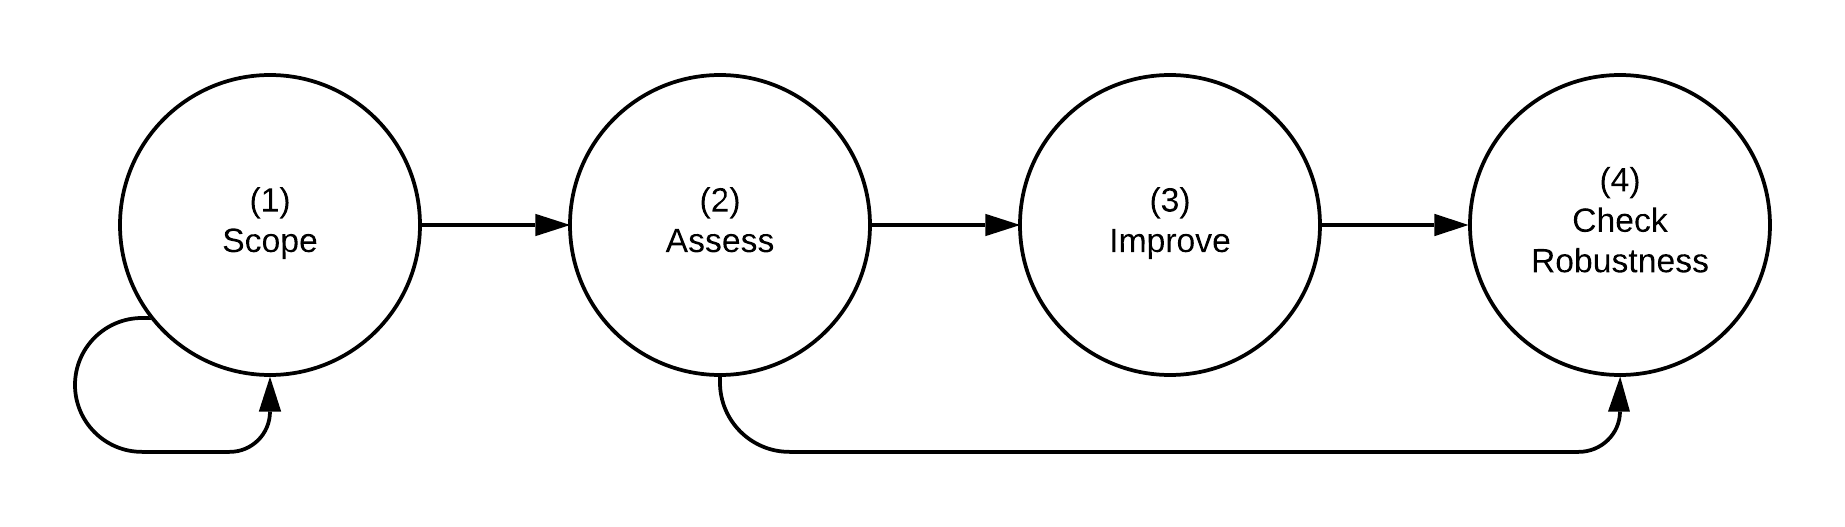
\includegraphics[width=1\linewidth]{stages}

\protect\hyperlink{scoping}{(1) Scoping}

\protect\hyperlink{assessment}{(2) Assessment}

\protect\hyperlink{improvements}{(3) Improvement}

\protect\hyperlink{robust}{(4) Robustness}

\protect\hyperlink{improvements}{Display-item-level}

\protect\hyperlink{paper-level}{Paper-level}

☐ Select paper

\protect\hyperlink{describe-inputs}{☐ Describe inputs}

\protect\hyperlink{rd}{☐ + Raw data}

\protect\hyperlink{paper-level}{☐ + Version control}

\protect\hyperlink{id-analy}{☐ Analytical choices}

\protect\hyperlink{check-acre}{☐ Check ACRE}

\protect\hyperlink{diagram}{☐ Reproduction diagrams}

\protect\hyperlink{ad}{☐ + Analysis data}

\protect\hyperlink{paper-level}{☐ + Documentation}

\protect\hyperlink{id-type}{☐ Type of choice}

☐ \protect\hyperlink{verify-rep-mat}{Check Rep.~pkg exists}

\protect\hyperlink{score}{☐ Reproduction score}

\protect\hyperlink{ac}{☐ + Analysis code}

\protect\hyperlink{paper-level}{☐ + Dynamic document}

\protect\hyperlink{id-val}{☐ Choice value}

\protect\hyperlink{read-summ}{☐ Read paper}

\protect\hyperlink{cc}{☐ + Cleaning code}

\protect\hyperlink{paper-level}{☐ + File structure}

\protect\hyperlink{test-rob}{☐ Justify and test alternatives}

\protect\hyperlink{declare-estimates}{☐ Declare estimates}

\protect\hyperlink{dac}{☐ Debug analysis code}

\protect\hyperlink{dcc}{☐ Debug cleaning code}

\href{https://berkeley.qualtrics.com/jfe/form/SV_2bO83uJvU9ZiTXv}{Record results in Survey 1}

\href{https://berkeley.qualtrics.com/jfe/form/SV_2gd9Y3XVtjLpZL7}{Record results in Survey 2}

\href{ADD\%20LINK}{Record results in Survey 3}

\hypertarget{intro}{%
\chapter*{Introduction}\label{intro}}
\addcontentsline{toc}{chapter}{Introduction}

In 2019, the \href{https://www.aeaweb.org/journals/policies/data-code/}{American Economic Association} updated its Data and Code Availability Policy to require that the AEA Data Editor verify the reproducibility of all papers before they are accepted by an AEA journal. In addition to the requirements laid out in the policy, several \href{https://aeadataeditor.github.io/aea-de-guidance/}{specific recommendations} were produced to facilitate compliance. This change in policy is expected to improve the computational reproducibility of all published research going forward, after several studies showed that rates of \emph{computational reproducibility} in economics at large range from somewhat low to alarmingly low \citep{galiani2018make, chang2015economics, kingi2018reproducibility}.

\emph{Replication}, or the process by which a study's hypotheses and findings are re-examined using different data or different methods (or both) \citep{King95} is an essential part of the scientific process that allows science to be ``self-correcting.'' \emph{Computational reproducibility}, or the ability to reproduce the results, tables, and other figures of a paper using the available data, code, and materials, is a necessary condition for replication. Computational reproducibility is assessed through the process of \emph{reproduction}. At the center of this process is the \emph{reproducer} (you!), a party rarely involved in the production of the original paper. Reproductions sometimes involve the \emph{original author} (whom we refer to as ``the author'') in cases where additional guidance and materials are needed to execute the process.

This exercise is designed for reproductions performed in economics graduate courses or undergraduate theses, with the goal of providing a common approach, terminology, and standards for conducting reproductions. The goal of reproduction, in general, is to assess and improve the computational reproducibility of published research in a way that facilitates further robustness checks, extensions, collaborations, and replication.

This exercise is part of the Accelerating Computational Reproducibility in Economics \href{https://www.bitss.org/ecosystem/acre/}{(ACRE)} project, which aims to assess, enable, and improve the computational reproducibility of published economics research. The ACRE project is led by the Berkeley Initiative for Transparency in the Social Sciences \href{https://bitss.org}{(BITSS)}---an initiative of the Center for Effective Global Action \href{https://cega.berkeley.edu/}{(CEGA)}---and Dr.~Lars Vilhuber, Data Editor for the journals of the American Economic Association (AEA). This project is supported by the Laura and John Arnold Foundation.

\hypertarget{beyond-binary-judgments}{%
\section*{Beyond binary judgments}\label{beyond-binary-judgments}}
\addcontentsline{toc}{section}{Beyond binary judgments}

Assessments of reproducibility can easily gravitate towards binary judgments that declare an entire paper ``reproducible'' or ``non-reproducible.'' These guidelines suggest a more nuanced approach by highlighting two realities that make binary judgments less relevant.

First, a paper may contain several scientific claims (or major hypotheses) that may vary in computational reproducibility. Each claim is tested using different methodologies, presenting results in one or more display items (outputs like tables and figures). Each display item will itself contain several specifications. Figure \ref{fig:diagram} illustrates this idea.

\begin{figure}
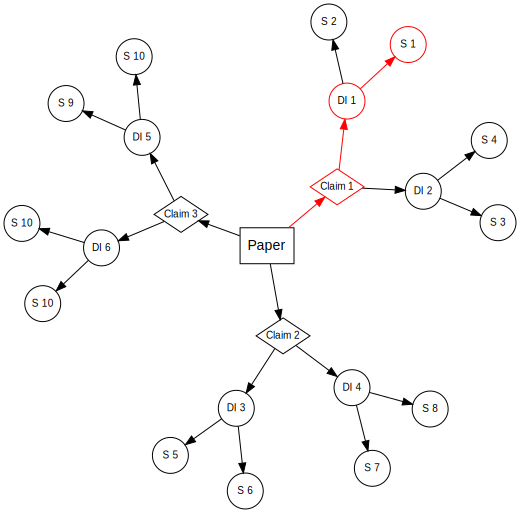
\includegraphics[width=1\linewidth]{paper-claims} \caption{One paper has multiple components to reproduce. <br> DI: Display Item, S: Specification }\label{fig:diagram}
\end{figure}

Second, for any given specification there are several levels of reproducibility, ranging from the absence of any materials to complete reproducibility starting from raw data. And even for a specific claim-specification, distinguishing the appropriate level can be far more constructive than simply labeling it as (ir)reproducible.

Note that the highest level of reproducibility, which requires complete reproducibility starting from raw data, is very demanding to achieve and should not be expected of all published research --- especially before 2019. Instead, this level can serve as an aspiration for the field of economics at large as it seeks to improve the reproducibility of research and facilitate the transmission of knowledge throughout the scientific community.

\hypertarget{stages-of-the-exercise}{%
\section*{Stages of the exercise}\label{stages-of-the-exercise}}
\addcontentsline{toc}{section}{Stages of the exercise}

This reproduction exercise is divided into four stages, corresponding to the first four chapters of these guidelines, with a fifth optional stage:

\begin{enumerate}
\def\labelenumi{\arabic{enumi}.}
\tightlist
\item
  \protect\hyperlink{scoping}{\textbf{Scoping}}, where you (the reproducer) will define the scope of the exercise by declaring a paper and the specific output(s) on which you will focus for the remainder of the exercise;\\
\item
  \protect\hyperlink{assessment}{\textbf{Assessment}}, where you will review and describe in detail the available reproduction package, and assess the current level of computational reproducibility of the selected outputs;
\item
  \protect\hyperlink{improvements}{\textbf{Improvement}}, where you will modify the content and/or the organization of the reproduction package to improve its reproducibility;\\
\item
  \protect\hyperlink{robust}{\textbf{Robustness checks}}, where you will assess the quality of selected analytical choices.
\end{enumerate}

These guidelines do not include a possible fifth stage of \textbf{Extension}. Here you may extend the current paper by including new methodologies or data. This step brings the reproduction exercise a step closer to \emph{replication}.

\begin{figure}
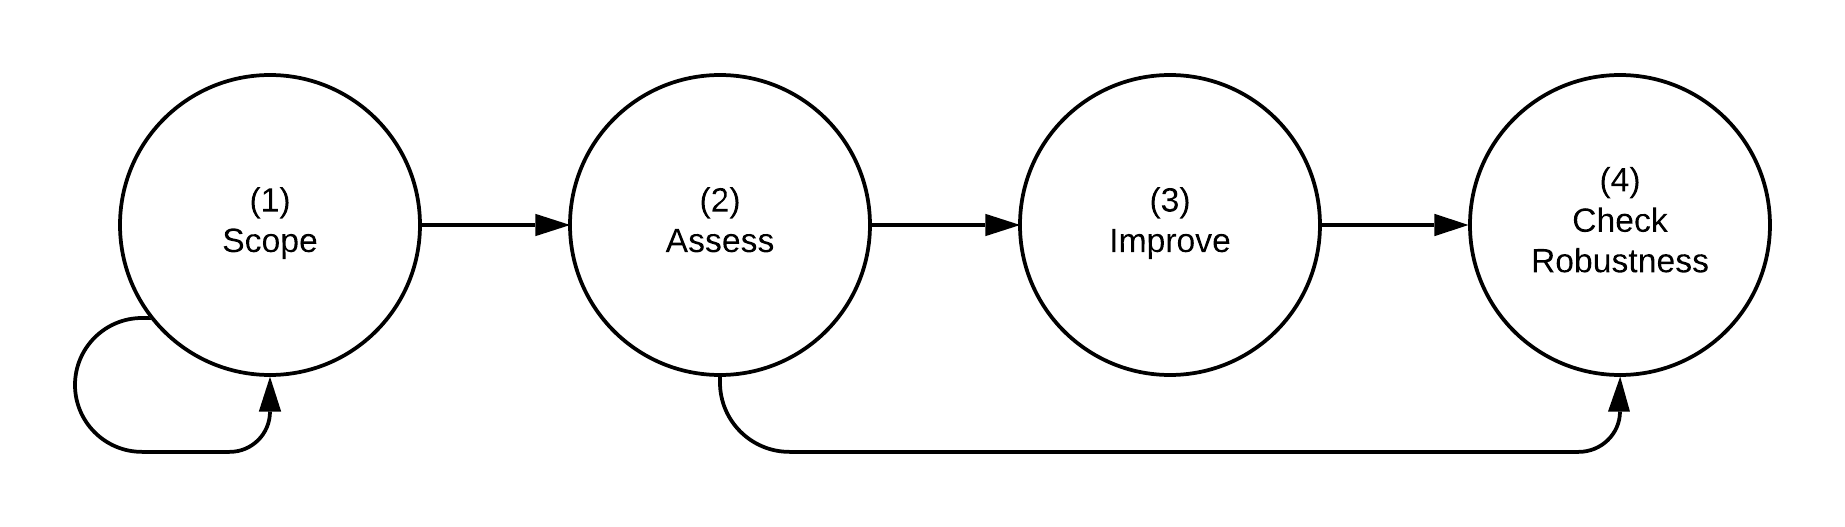
\includegraphics[width=1\linewidth]{stages} \caption{One paper has multiple components to reproduce. <br> DI: Display Item, S: Specification}\label{fig:stages-intro}
\end{figure}

\label{tab:stages-intro}Relative Level of Effort by Type of exercise

Exercise

Scope

Assess

Improve

Robust

Graduate course

10\%

35\%

25\%

30\%

Graduate research

5\%

25\%

40\%

30\%

Undergrad thesis

5\%

20\%

50\%

25\%

Table \ref{tab:stages-intro} depicts suggested levels of effort for each stage of the exercise depending on the context in which you are performing a reproduction. This process need not be chronologically linear. For example, you may realize that the scope of a reproduction is too ambitious and switch to a less intensive one. Later in the exercise, you can also begin testing different specifications for robustness while also assessing a paper's level of reproducibility.

\hypertarget{recording-the-results-of-the-exercise}{%
\section*{Recording the results of the exercise}\label{recording-the-results-of-the-exercise}}
\addcontentsline{toc}{section}{Recording the results of the exercise}

You will be asked to record the results of your reproduction as you progress through each stage.

In \emph{Stage 1: \protect\hyperlink{scoping}{Scoping}}, complete \textbf{\href{https://berkeley.qualtrics.com/jfe/form/SV_2bO83uJvU9ZiTXv}{Survey 1}}, where you will declare your paper of choice and the specific display item(s) and specifications on which you will focus for the remainder of the exercise. This step may also involve writing a brief 1-2 page summary of the paper (depending on your instructor or goals).

In \emph{Stage 2: \protect\hyperlink{assessment}{Assessment}}, you will inspect the paper's reproduction package (raw data, analysis data, and code), connect the display item to be reproduced with its inputs, and assign a reproducibility score to each output.

In \emph{Stage 3: \protect\hyperlink{improvements}{Improvement}}, you will try to improve the reproducibility of the selected outputs by adding missing files, documentation, and report any potential changes in the level of reproducibility. Use \textbf{Survey 2} to record your work at Stages 2 and 3 (you will receive access instructions for Survey 2 when you submit Survey 1).

In \emph{Stage 4: \protect\hyperlink{robust}{Robustness Checks}}, you will assess different analytical choices and test possible variations. Use \textbf{Survey 3} to record your work at this stage.

\hypertarget{reproduction-strategies}{%
\section*{Reproduction Strategies}\label{reproduction-strategies}}
\addcontentsline{toc}{section}{Reproduction Strategies}

Generally, a reproduction will begin with a thorough reading of the study being reproduced. However, subsequent steps may follow from a \emph{reproduction strategy}. For example, a reproduction may closely follow the order of the steps outlined above. This might entail the reproducer first choosing a set of results whose production they are interested in assessing or understanding, completely reproducing these results to the extent possible, and then making modifications to the reproduction package. Another potential strategy could be for the reproducer to develop potential robustness checks or extensions while reading the study, which would lead to the definition of a set of results to be assessed via reproduction. Yet another reproduction strategy may be for the reproducer to seek out a paper that uses a particular dataset to which they have access or an interest in using, reproducing the results that use that dataset as an input, then probing the robustness of the results to various data cleaning decisions.

The various uses of reproduction makes the number of potential reproduction strategies quite large. In choosing or designing a reproduction strategy, it is helpful to clearly identify the goal of the reproduction. In all of the examples laid out in the paragraph above, the order in which the steps of the reproduction exercise are taken is at least partially determined by what the reproducer hopes to get from the exercise. The structure provided in these guidelines, together with a clear reproduction goal, can facilitate the implementation of an efficient reproduction strategy.

\hypertarget{scoping}{%
\chapter{Scoping}\label{scoping}}

The goal of this stage is to help you define the scope of your exercise by declaring a paper and the specific output(s) on which you will focus. You might first consider multiple papers without analyzing them more closely (we refer to these as \textbf{candidate papers}) before moving forward with your \textbf{declared paper}.

It is likely that you will choose a declared paper based on whether or not you can locate its reproduction package. A \textbf{reproduction package} is the collection of materials that make it possible to reproduce a paper. This package may contain data, code, or documentation. If you are unable to independently locate the reproduction package for your paper, you can ask the paper's author for it (find guidance on this in \href{https://bitss.github.io/ACRE/guidance-for-a-constructive-exchange-between-reproducers-and-original-authors.html}{Chapter 5}) or simply choose another candidate paper. If you still want to explore the reproducibility of a paper with no reproduction package, these guidelines provide instructions for requesting materials from authors to create a public reproduction package, or if this proves unsuccessful, for building your reproduction package from scratch.

To avoid duplicating the efforts of others who may be interested in reproducing one of your candidate papers, \textbf{we ask that you record your candidate papers in the ACRE database} (currently under development).

Note that in this stage, \emph{you are not expected to review the reproduction materials in detail}, as you will dedicate most of your time to this in later stages of the exercise. If materials are available, you will read the paper and declare the scope of the reproduction exercise. You can expect to spend between 1-3 days in this Scoping stage, though this may vary based on the length and the complexity of the paper, and the availability of reproduction materials.

\textbf{\emph{Use \href{https://berkeley.qualtrics.com/jfe/form/SV_2bO83uJvU9ZiTXv}{Survey 1} to record your work in this stage.}}

\hypertarget{from-candidate-to-declared-paper}{%
\section{From candidate to declared paper}\label{from-candidate-to-declared-paper}}

At this point of the exercise, you are \emph{only validating the availability} of (at least) one reproduction package and not assessing the quality of its content. Follow the steps below to verify that a reproduction package is available, and stop whenever you find it (this may mean mean that you have found your declared paper).

\begin{enumerate}
\def\labelenumi{\arabic{enumi}.}
\tightlist
\item
  Check whether previous reproduction attempts have beeen recorded in the ACRE Database for the paper (more on the ACRE Database in the next section).
\item
  Check the journal or publisher's website, looking for materials named ``Data and Materials,'' ``Supplemental Materials,'' ``Reproduction/Replication Package/Materials,'' etc.\\
\item
  Look for links in the paper (review the footnotes and appendices).\\
\item
  Review the personal websites of the paper's author(s).
\item
  Contact the author(s) to request the reproduction package using \href{https://bitss.github.io/ACRE/guidance-for-a-constructive-exchange-between-reproducers-and-original-authors.html\#contacting-the-original-authors-when-there-is-no-reproduction-package}{this} email template. In this and future interactions with authors, we encourage you to follow our guidance outlined in \href{https://bitss.github.io/ACRE/guidance-for-a-constructive-exchange-between-reproducers-and-original-authors.html\#contacting-the-original-authors-when-there-is-no-reproduction-package}{Chapter 5}.
\item
  Deposit the reproduction package in a trusted repository (e.g., \href{https://dataverse.org/}{Dataverse}, \href{https://www.openicpsr.org/openicpsr/}{Open ICPSR}, \href{https://zenodo.org/}{Zenodo}, or the \href{https://osf.io/}{Open Science Framework}) under the name \texttt{Original\ reproduction\ package\ for\ -\ Title\ of\ the\ paper}. You will be asked to provide the URL of the repository in Survey 1.
\end{enumerate}

In case you need to contact the authors, make sure to \emph{allocate sufficient time for this step} (we suggest at least three weeks before the date you plan to start the reproduction). Instructors should also plan to accordingly (e.g., if the ACRE exercise is expected to take place in the middle of the semester, students should review candidate papers and (if applicable) contact the authors in the first few weeks of the semester).

Review the decision tree (Figure \#) below for a more detailed overview of this process. Remember, \emph{if at any step of the process you decide to abandon the paper, make sure to record the candidate paper in the ACRE database} before moving on to another candidate paper. Once you have obtained the reproduction package, the \emph{candidate paper} becomes your \emph{declared paper} and you can move forward with the exercise! Do not invest time in doing a detailed read of any paper until you are sure that it is your declared paper.

\hypertarget{candidate-paper-entries-in-the-acre-database}{%
\subsection{Candidate paper entries in the ACRE Database}\label{candidate-paper-entries-in-the-acre-database}}

If the ACRE database contains previous reproduction attempts of the paper, you will see a report card with the following information:

\begin{quote}
\textbf{Box 1:} Summary Report Card for ACRE Paper Entry\\
\textbf{Title:} Sample Title\\
\textbf{Authors:} Jane Doe \& John Doe\\
\textbf{Original Reproduction Package Available:} URL/No {[}What does this mean? Add some context{]}.
{[}If ``No''{]} \textbf{Contacted Authors?:} Yes/No\\
{[}If ``Yes(contacted)''{]} \textbf{Type of Response:} Categories (6).\\
\textbf{Additional Reproduction Packages:} Number (eg., 2)\\
\textbf{Authors Available for Further Questions for ACRE Reproductions:} Yes/No/Unknown\\
\textbf{Open for reproductions:} Yes/No {[}Same as above: what does this mean? Add more context{]}.
\end{quote}

If after taking steps 1-5 above (or for some other reason) you are unable to locate the reproduction package, record your candidate paper (and if applicable, the outcome of your correspondence with the original authors) in the ACRE database following the example above.

View Decision Tree To Select Paper

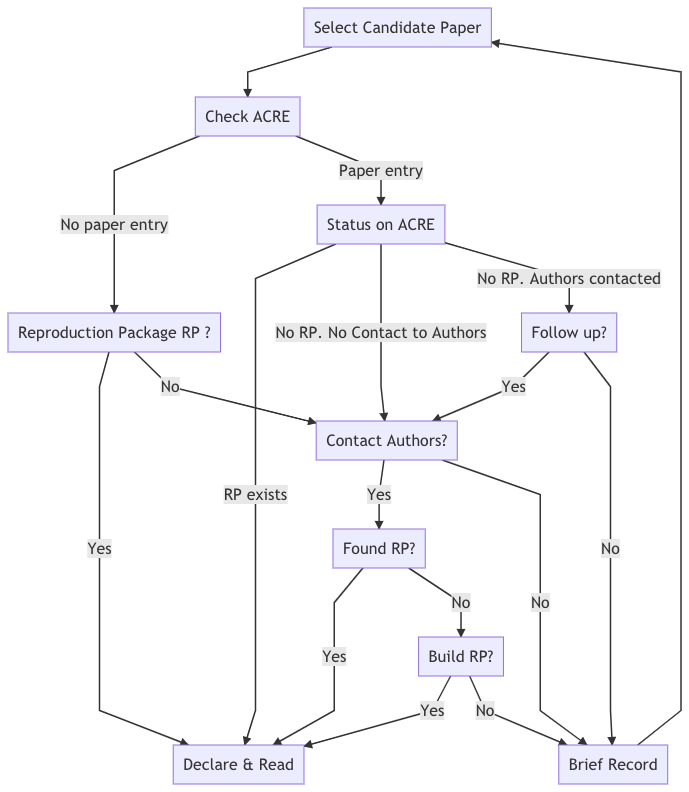
\includegraphics{candidate-to-declared-paper.png}

\hypertarget{scoping-your-declared-paper}{%
\section{Scoping your declared paper}\label{scoping-your-declared-paper}}

Once you have identified your declared paper, get familiarized with it and choose the specific output(s) on which you will focus for the remainder of the exercise.

\hypertarget{read-sum}{%
\subsection{Read and summarize the paper}\label{read-sum}}

Depending on how much time you have, we recommend that you write a short (1-2 page) summary of the paper. This will help remind you of the key elements to focus on for the reproduction, and demonstrate your understanding of the paper (for yourself and others like your instructor or advisor).

When reading or summarizing the paper, try to answer the following questions:

\begin{itemize}
\tightlist
\item
  Would you classify the paper's scientific claims as mainly focused on estimating a causal relationship, estimating/predicting a descriptive statistic of a population, or something else?
\item
  How many scientific claims (descriptive or causal) are investigated in the paper?
\item
  What is the population for which the estimates apply?
\item
  What is the population that is the focus of the paper as a whole?
\item
  What are the main data sources used in the paper?
\item
  How many display items are there in the paper (tables, figures, and inline results)?\\
\item
  What is the main statistical or econometric method used to examine each claim?
\item
  What is the author's preferred specification (or yours, if the authors are not clear)?
\item
  What are some robustness checks for the preferred specification?
\end{itemize}

\hypertarget{declare-estimates}{%
\subsection{Record scope of the exercise}\label{declare-estimates}}

By now you should have a fairly good understanding of the paper's content. You do not, however, need to have spent any time reviewing the reproduction package in detail.

At this point, you should clearly specify which part of the paper will be the main focus of your reproduction. Focus on specific estimates, represented by a unique combination of claim-display item-specification as represented in figure \ref{fig:diagram}. If you plan to scope more than one claim, \emph{we strongly recommend starting with just one} and recording your results. You can then initiate another record in ACRE later for the second (or third, fourth, etc.) claim to reproduce using the materials and knowledge you developed in the first exercise. You can, however, reproduce more than one claim if you are already familiar with the paper.

In the Assessment stage, the reproduction will be centered around the display item(s) that contain the specification you indicate at this point.

\hypertarget{declare-specific-main-estimates-to-reproduce.}{%
\subsubsection*{Declare specific main estimates to reproduce.}\label{declare-specific-main-estimates-to-reproduce.}}
\addcontentsline{toc}{subsubsection}{Declare specific main estimates to reproduce.}

Identify a scientific claim and its corresponding preferred specification, and record its magnitude, standard error, and location in the paper (page, table \#, and table row and column). If the authors did not explicitly chose a particular estimate, you will be asked to select one. In addition to the preferred estimate, reproduce up to five estimates that correspond to alternative specifications of the preferred estimate.

\hypertarget{declare-possible-robustness-checks-for-main-estimates-optional.}{%
\subsubsection*{Declare possible robustness checks for main estimates (optional).}\label{declare-possible-robustness-checks-for-main-estimates-optional.}}
\addcontentsline{toc}{subsubsection}{Declare possible robustness checks for main estimates (optional).}

After reading the paper, you might wonder why the authors did not conduct a specific robustness test. If you think that such analysis could have been done \emph{within the same methodology} and \emph{using the same data} (e.g., by including or excluding a subset of the data like ``high-school dropouts'' or ``women''), please specify a robustness test that you would like to conduct before starting the Assessment stage.

These are the elements you will need for the Scoping stage. \textbf{You now have all the elements necessary to complete \href{https://berkeley.qualtrics.com/jfe/form/SV_2bO83uJvU9ZiTXv}{Survey 1}.}

\begin{center}\rule{0.5\linewidth}{0.5pt}\end{center}

\hypertarget{identify-your-relevant-timeline.}{%
\section{Identify your relevant timeline.}\label{identify-your-relevant-timeline.}}

Before you begin working on the three main stages of the reproduction exercise (Assessment, Improvement, and Robustness), it is important to manage your own expectations and those of your instructor or advisor. Be mindful of your time limitations when defining the scope of your reproduction activity. These will depend on the type of exercise chosen by your instructor or advisor and may vary from a weeklong homework assignment, to a longer class project that may take a month to complete or a semester-long project (an undergraduate thesis, for example).

Table 1 shows an example distribution of time across three different reproduction formats. The Scoping and Assessment stages are expected to last roughly the same amount of time across all formats (lasting longer for the semester-long activities, and acknowledgin that less experienceed researchers, such as undergraduate students, may need more time). Differences emerge in the distribution of time for the last two main stages: Improvements and Robustness. For shorter exercises, we recommend avoiding any possible improvements to the raw data (or cleaning code). This will limit how many robustness checks are possible (for example, by limiting your ability to reconstruct variables according to slightly different definitions), but it should leave plenty of time for testing different specifications at the analysis level.

2 weeks (\textasciitilde10 days)

1 month (\textasciitilde20 days)

1 semester (\textasciitilde100 days)

analysis data

raw data

analysis data

raw data

analysis data

raw data

Scoping

10\% (1 day)

5\% (1 day)

5\% (5 days)

Assessment

35\%

25\%

15\%

Improvement

25\%

0\%

40\%

20\%

30\%

Robustness

25\%

5\%

25\%

25\%

\hypertarget{assessment}{%
\chapter{Assessment}\label{assessment}}

In this stage, you will review and describe in detail the available reproduction materials, and assess levels of computational reproducibility for the selected outputs, as well as for the overall paper. This stage is designed to record as much of the learning process behind a reproduction as possible to facilitate incremental improvements, and allow future reproducers to pick up easily where others have left off.

First, you will provide a detailed description of the reproduction package. Second, you will connect the outputs you've chosen to reproduce with their corresponding inputs. With these elements in place, you can score the level of reproducibility of each output, and report on paper-level dimensions of reproducibility.

In the \emph{Scoping} stage, you declared a paper, identified the specific claims you will reproduce, and recorded the main estimates that support the claims. In this stage, you will identify all outputs that contain those estimates. You will also decide if you are interested in assessing the reproducibility of that entire output (e.g., ``Table 1''), or will assess only a pre-specified estimates (e.g., ``rows 3 and 4 of Table 1''). Additionally, you can include other outputs of interest.

\textbf{Use \emph{Survey 2} to record your work as part of this step.}

\emph{Tip:} We recommend that you first focus on one specific output (e.g., ``Table 1''). After completing the assessment for this output, you will have a much easier time translating improvements to other outputs.

\hypertarget{describe-inputs}{%
\section{Describe the inputs.}\label{describe-inputs}}

This section explains how to list \emph{all} input materials found or referred to in the reproduction package. First, you will identify data sources and connect them with their raw data files (when available). Second, you will locate and provide a brief description of the analytic data files. Finally, you will locate, inspect, and describe the analytic code used in the paper.

The following terms will be used in this section:

\begin{itemize}
\item
  \textbf{Cleaning code:} A script associated primarily with data cleaning. Most of its content is dedicated to actions like deleting variables or observations, merging data sets, removing outliers, or reshaping the structure of the data (from long to wide, or vice versa).
\item
  \textbf{Analysis code:} A script associated primarily with analysis. Most of its content is dedicated to actions like running regressions, running hypothesis tests, computing standard errors, and imputing missing values.
\end{itemize}

\hypertarget{desc-sourc}{%
\subsection{Describe the data sources and raw data.}\label{desc-sourc}}

In the paper you chose, find references to all \emph{data sources} used in the analysis. A data source is usually described in narrative form. For example, if in the body of the paper you see text like ``\ldots for earnings in 2018 we use the Current Population Survey\ldots{}'', the data source is ``Current Population Survey 2018''. If it is mentioned for the first time on page 1 of the Appendix, its location should be recorded as ``A1''. Do this for all the data sources mentioned in the paper.

Data sources also vary by unit of analysis, with some sources matching the same unit of analysis used in the paper (as in previous examples), while others are less clear (e.g., ``our information on regional minimum wages comes from the Bureau of Labor Statistics.'' This should be recorded as ``regional minimum wages from the Bureau of Labor Statistics'').

Next, look at the reproduction package and map the \emph{data sources} mentioned in the paper to the \emph{data files} in the available materials. Record their folder locations relative to the main reproduction folder\footnote{a relative location takes the form of \texttt{/folder\_in\_rep\_materials/sub\_folder/file.txt}, in contrast to an absolute location that takes the form of \texttt{username/documents/projects/repros/folder\_in\_rep\_materials/sub\_folder/file.txt}}. In addition to looking at the existing data files, we recommend that you review the first lines of all code files (especially cleaning code), looking for lines that call the datasets. Inspecting these scripts may help you understand how different data sources are used, and possibly identify any files that are missing from the reproduction package.

Record this information in this \href{https://docs.google.com/spreadsheets/d/1LUIdVFH0OfR70C7z07TYeE-uWzKI_JIeWUMaYhqEKK0/edit\#gid=0\&range=A1}{standardized spreadsheet} (download it or make a copy for yourself), using the following structure:\\

\label{tab:raw-data-information}Raw data information

data\_source

page

data\_files

known\_missing

directory

``Current Population Survey 2018''

A1

cepr\_march\_2018.dta

/data/

``DHS 2010 - 2013''

4

nicaraguaDHS\_2010.csv; boliviaDHS2010.csv; nicaraguaDHS\_2011.csv; nicaraguaDHS\_2012.csv; boliviaDHS\_2012.csv; nicaraguaDHS\_2013.csv; boliviaDHS\_2013.csv

boliviaDHS\_2011.csv

/rawdata/DHS/

``2017 SAT scores''

4

Not available

/data/to\_clean/

\ldots{}

\ldots{}

\ldots{}

\ldots{}

\ldots{}

\begin{verbatim}
      Raw data information:
      |----------------------|------|-----------------------------------------------|---------------------|---------------------|
      | data_source          | page | data_files                                    | known_missing       | directory           |
      |----------------------|------|-----------------------------------------------|---------------------|---------------------|
      | "Current Population  | A1    | cepr_march_2018.dta                          |                     | \data\              |
      | Survey 2018"         |      |                                               |                     |                     |
      |----------------------|------|-----------------------------------------------|---------------------|---------------------|
      | "DHS 2010 - 2013"    | 4    | nicaraguaDHS_2010.csv;                        | boliviaDHS_2011.csv | \rawdata\DHS\       |
      |                      |      | boliviaDHS_2010.csv; nicaraguaDHS_2011.csv;   |                     |                     |
      |                      |      | nicaraguaDHS_2012.csv; boliviaDHS_2012.csv;   |                     |                     |
      |                      |      | nicaraguaDHS_2013.csv; boliviaDHS_2013.csv    |                     |                     |
      |----------------------|------|-----------------------------------------------|---------------------|---------------------|
      | "2017 SAT scores"    | 4    | Not available                                 |                     | \data\to_clean\     |
      |----------------------|------|-----------------------------------------------|---------------------|---------------------|
      | ...                  | ...  | ...                                           | ...                 | ...                 |
      |----------------------|------|-----------------------------------------------|---------------------|---------------------|
\end{verbatim}

\textbf{Note:} lists if files in the data\_files and known\_missing columns should have entries separated by a semi-colon to for the spreadsheet to be compatible with the ACRE Diagram Builder.

\hypertarget{desc-analy}{%
\subsection{Describe the analytic data sets.}\label{desc-analy}}

List all the analytic files you can find in the reproduction package, and identify their locations relative to the main reproduction folder. Record this information in the \href{https://docs.google.com/spreadsheets/d/1LUIdVFH0OfR70C7z07TYeE-uWzKI_JIeWUMaYhqEKK0/edit\#gid=1299317837\&range=A1}{standardized spreadsheet}.

As you progress through the exercise, add to the spreadsheet a one-line description of each file's main content (for example: \texttt{all\_waves.csv} has the simple description \texttt{data\ for\ region-level\ analysis}). This may be difficult in an initial review, but will become easier as you go along.

The resulting report will have the following structure:

\label{tab:analysis-data-information}Analysis data information

analysis\_data

location

description

final\_data.csv

/analysis/fig1/

data for figure1

all\_waves.csv

/final\_data/v1\_april/

data for region-level analysis

\ldots{}

\ldots{}

\ldots{}

\begin{verbatim}
      Analysis data information:
      |----------------|-----------------------|--------------------------------|
      | analysis_data  | location              | description                    |
      |----------------|-----------------------|--------------------------------|
      | final_data.csv | /analysis/fig1/       | data for figure1               |
      |----------------|-----------------------|--------------------------------|
      | all_waves.csv  | /final_data/v1_april/ | data for region-level analysis |
      |----------------|-----------------------|--------------------------------|
      | ...            | ...                   | ...                            |
      |----------------|-----------------------|--------------------------------|
\end{verbatim}

\hypertarget{desc-scripts}{%
\subsection{Describe the code scripts.}\label{desc-scripts}}

List all code files that you found in the reproduction package and identify their locations relative to the master reproduction folder. Review the beginning and end of each code file and identify the inputs required to successfully run the file. Inputs may include data sets or other code scripts that are typically found at the beginning of the script (e.g., \texttt{load}, \texttt{read}, \texttt{source}, \texttt{run}, \texttt{do} ). For each code file, record all inputs together and separate each item with ``;''. Outputs may include other datasets, figures, or plain text files that are typically at the end of a script (e.g., \texttt{save}, \texttt{write}, \texttt{export}). For each code file, record all outputs together and separate each item with ``;''. Provide a one-line description of what each code file does. Record all of this information in the \href{https://docs.google.com/spreadsheets/d/1LUIdVFH0OfR70C7z07TYeE-uWzKI_JIeWUMaYhqEKK0/edit\#gid=1617799822\&range=A1}{standardized spreadsheet}, using the following structure:

\label{tab:code-files-information}Code files information

file\_name

location

inputs

outputs

description

primary\_type

output\_table1.do

/code/analysis/

analysis\_data01.csv

output1\_part1.txt

produces first part of table 1 (unformatted)

analysis

data\_cleaning02.R

/code/cleaning

admin\_01raw.csv

analysis\_data02.csv

removes outliers and missing vals from raw admin data

cleaning

\ldots{}

\ldots{}

\ldots{}

\ldots{}

\ldots{}

\ldots{}

\begin{verbatim}
      Code files information:
      |-------------------|------------------|---------------------|---------------------|----------------------|--------------|
      | file_name         | location         | inputs              | outputs             | description          | primary_type |
      |-------------------|------------------|---------------------|---------------------|----------------------|--------------|
      | output_table1.do  | /code/analysis/  | analysis_data01.csv | output1_part1.txt   | produces first part  | analysis     |
      |                   |                  |                     |                     | of table 1           |              |
      |                   |                  |                     |                     | (unformatted)        |              |
      |-------------------|------------------|---------------------|---------------------|----------------------|--------------|
      | data_cleaning02.R | /code/cleaninig/ | admin_01raw.csv     | analysis_data02.csv | removes outliers     | cleaning     |
      |                   |                  |                     |                     | and missing vals     |              |
      |                   |                  |                     |                     | from raw admin data  |              |
      |-------------------|------------------|---------------------|---------------------|----------------------|--------------|
      | ...               | ...              | ...                 | ...                 | ...                  | ...          |
      |-------------------|------------------|---------------------|---------------------|----------------------|--------------|
\end{verbatim}

As you gain an understanding of each code script, you will likely find more inputs and outputs -- we encourage you to update the \href{https://docs.google.com/spreadsheets/d/1LUIdVFH0OfR70C7z07TYeE-uWzKI_JIeWUMaYhqEKK0/edit\#gid=1617799822\&range=A1}{standardized spreadsheet}. Once finished with the reproduction exercise, classify each code file as \emph{analysis} or \emph{cleaning}. We recognize that this may involve subjective judgment, so we suggest that you conduct this classification based on each script's main role.

\textbf{Note:} If a code script takes multiple inputs and/or produces multiple outputs they should be listed as semicolon separated lists in order to be compatible with the ACRE Diagram Builder.

\hypertarget{diagram}{%
\section{Connect each output to all its inputs}\label{diagram}}

Using the information collected above, you can trace your output-to-be-reproduced to its primary sources. Email the standardized spreadsheets from above (sections \ref{desc-sourc}, \ref{desc-analy} and \ref{desc-scripts}) to the ACRE Diagram Builder at \href{mailto:acre@berkeley.edu}{\nolinkurl{acre@berkeley.edu}}. You should receive an email within 24 hours with a reproduction diagram tree that represents the information available on the workflow behind a specific output.

\hypertarget{complete-workflow-information}{%
\subsection{Complete workflow information}\label{complete-workflow-information}}

If you were able to identify all the relevant components in the previous section, the ACRE Diagram Builder will produce a tree diagram that looks similar to the one below.

\begin{verbatim}
    table1.tex
        |___[code] analysis.R
            |___analysis_data.dta
                |___[code] final_merge.do
                    |___cleaned_1_2.dta
                    |   |___[code] clean_merged_1_2.do
                    |       |___merged_1_2.dta
                    |           |___[code] merge_1_2.do
                    |               |___cleaned_1.dta
                    |               |   |___[code] clean_raw_1.py
                    |               |       |___raw_1.dta
                    |               |___cleaned_2.dta
                    |                   |___[code] clean_raw_2.py
                    |                       |___raw_2.dta
                    |___cleaned_3_4.dta
                        |___[code] clean_merged_3_4.do
                            |___merged_3_4.dta
                                |___[code] merge_3_4.do
                                    |___cleaned_3.dta
                                    |   |___[code] clean_raw_3.py
                                    |       |___raw_3.dta
                                    |___cleaned_4.dta
                                        |___[code] clean_raw_4.py
                                            |___raw_4.dta
\end{verbatim}

This diagram, built with the information you provided, is already an important contribution to understanding the necessary components required to reproduce a specific output. It summarizes key information to allow for more constructive exchanges with original authors or other reproducers. For example, when contacting the authors for guidance, you can use the diagram to point out specific files you need. Formulating your request this way makes it easier for authors to respond and demonstrates that you have a good understanding of the reproduction package.

\hypertarget{incomplete-workflow-information}{%
\subsection{Incomplete workflow information}\label{incomplete-workflow-information}}

In many cases, some of the components of the workflow will not be easily identifiable (or missing) in the reproduction package. Here the Diagram Builder will return a partial reproduction tree diagram. For example, if the files \texttt{merge\_1\_2.do}, \texttt{merge\_3\_4.do}, and \texttt{final\_merge.do} are missing from the previous diagram, the ACRE Diagram Builder will produce the following diagram:

\begin{verbatim}
    cleaned_3.dta
        |___[code] clean_raw_3.py
            |___raw_3.dta

    table1.tex
        |___[code] analysis.R
            |___analysis_data.dta

    cleaned_3_4.dta
        |___[code] clean_merged_3_4.do
            |___merged_3_4.dta

    cleaned_1.dta
        |___[code] clean_raw_1.py
            |___raw_1.dta

    cleaned_2.dta
        |___[code] clean_raw_2.py
            |___raw_2.dta

    cleaned_4.dta
        |___[code] clean_raw_4.py
            |___raw_4.dta

    cleaned_1_2.dta
        |___[code] clean_merged_1_2.do
            |___merged_1_2.dta
    Unused data sources: None.
\end{verbatim}

In this case, you can still manually combine this partial information with your knowledge from the paper and own judgement to produce a ``candidate'' tree diagram (which might lead to different reproducers recreating different diagrams). This may look like the following:

\begin{verbatim}
    table1.tex
        |___[code] analysis.R
            |___analysis_data.dta
                |___MISSSING CODE FILE(S) #3
                    |___cleaned_3_4.dta
                    |       |___[code] clean_merged_3_4.do
                    |           |___merged_3_4.dta
                    |               |___MISSSING CODE FILE(S) #2
                    |                   |___cleaned_3.dta
                    |                   |       |___[code] clean_raw_3.py
                    |                   |           |___raw_3.dta    
                    |                   |___cleaned_4.dta
                    |                           |___[code] clean_raw_4.py
                    |                               |___raw_4.dta
                    |___cleaned_1_2.dta
                            |___[code] clean_merged_1_2.do
                                |___merged_1_2.dta
                                    |___MISSSING CODE FILE(S) #1
                                        |___cleaned_1.dta
                                        |       |___[code] clean_raw_1.py
                                        |           |___raw_1.dta
                                        |   
                                        |___cleaned_2.dta
                                                |___[code] clean_raw_2.py
                                                    |___raw_2.dta
\end{verbatim}

To leave a record of the reconstructed diagrams, you will have to amend the input spreadsheets using placeholders for the missing components. In the example above, you should add the following entries to the code description spreadsheet:

\label{tab:adding-rows}Adding rows to code spreadsheet

file\_name

location

inputs

outputs

description

primary\_type

\ldots{}

\ldots{}

\ldots{}

\ldots{}

\ldots{}

\ldots{}

missing\_file1

unknown

cleaned\_1.dta, cleaned\_2.dta

merged\_1\_2.dta

missing code

unknown

missing\_file2

unknown

cleaned\_3.dta, cleaned\_4.dta

merged\_3\_4.dta

missing code

unknown

missing\_file3

unknown

merged\_3\_4.dta, merged\_1\_2.dta

analysis\_data.dta

missing code

unknown

\begin{verbatim}
    Adding rows to code spreadsheet:
    |-------------------|------------------|---------------------|---------------------|----------------------|--------------|
    | file_name         | location         | inputs              | outputs             | description          | primary_type |
    |-------------------|------------------|---------------------|---------------------|----------------------|--------------|
    | ...               | ...              | ...                 | ...                 | ...                  | ...          |
    |-------------------|------------------|---------------------|---------------------|----------------------|--------------|
    | missing_file1     | unknown          | cleaned_1.dta;      | merged_1_2.dta      | missing code         | unknown      |
    |                   |                  | cleaned_2.dta       |                     |                      |              |
    |-------------------|------------------|---------------------|---------------------|----------------------|--------------|
    | missing_file2     | unknown          | cleaned_3.dta;      | merged_3_4.dta      | missing code         | unknown      |
    |                   |                  | cleaned_4.dta       |                     |                      |              |                  
    |-------------------|------------------|---------------------|---------------------|----------------------|--------------|
    | missing_file3     | unknown          | merged_3_4.dta;    | analysis_data.dta   | missing code         | unknown      |
    |                   |                  | merged_1_2.dta     |                     |                      |              |                  
    |-------------------|------------------|---------------------|---------------------|----------------------|--------------|
\end{verbatim}

As in the cases with complete workflows, these diagrams (fragmented or reconstructed trees) provide important information for assessing and improving the reproducibility of specific outputs. Reproducers can compare reconstructed trees and/or contact original authors with highly specific inquiries.

For more examples of diagrams connecting final outputs to initial raw data, \protect\hyperlink{additional-diagrams}{see here}.

\hypertarget{unused-data-sources}{%
\subsection{Unused Data Sources}\label{unused-data-sources}}

It is possible that not all data included in a replication package are actually used in code scripts in the reproduction package. This would be the case if, for example, the raw data and analysis data are included, but not the script that generates the analysis data. As a concrete example, consider what the original diagram above would look like if the only code included in the reproduction package were analysis.R:

\begin{verbatim}
    table1.tex
        |___[code] analysis.R
            |___analysis_data.dta

    Unused data sources:
    raw_1.dta
    raw_2.dta
    raw_3.dta
    raw_4.dta

    Unused analysis data:
    cleaned_1.dta
    cleaned_2.dta
    cleaned_3.dta
    cleaned_4.dta
    merged_1_2.dta
    merged_3_4.dta
    cleaned_1_2.dta
    cleaned_3_4.dta
\end{verbatim}

In this case, there are many data files that were listed in the raw data and analytic data spreadsheets that are not used by any code script in the replication package.

\hypertarget{score}{%
\section{Assign a reproducibility score.}\label{score}}

Once you have identified all possible inputs and have a clear understanding of the connection between the outputs and inputs, you can start to assess the output-specific level of reproducibility.

Take note of the following concepts in this section:

\begin{itemize}
\item
  \textbf{Computationally Reproducible from Analytic data (CRA):} The output can be reproduced with minimal effort starting from the \emph{analytic} datasets.
\item
  \textbf{Computationally Reproducible from Raw data (CRR):} The output can be reproduced with minimal effort from the \emph{raw} datasets.
\item
  \textbf{Minimal effort:} One hour or less is required to run the code, not including computing time.
\end{itemize}

\hypertarget{levels-of-computational-reproducibility-for-a-specific-output}{%
\subsection{Levels of Computational Reproducibility for a Specific Output}\label{levels-of-computational-reproducibility-for-a-specific-output}}

Each level of computational reproducibility is defined by the availability of data and materials, and whether or not the available materials faithfully reproduce the output of interest. The description of each level also includes possible improvements that can help advance the reproducibility of the output to a higher level. You will learn in more detail about the possible improvements.

Note that the assessment is made \emph{at the output level} -- a paper can be highly reproducible for its main results, but suffer from low reproducibility for other outputs. The assessment includes a 10-point scale, where 1 represents that, under current circumstances, reproducers cannot access any reproduction package, while 10 represents access to all the materials and being able to reproduce the target outcome from the raw data.

\begin{itemize}
\tightlist
\item
  \textbf{Level 1 (L1):} No data or code are available. Possible improvements include adding: raw data (+AD), analysis data (+RD), cleaning code (+CC), and analysis code (+AC).
\end{itemize}

You will have detected papers that are reproducible at Level 1 as part of the Scoping stage (unsuccessful candidate papers). Make sure to take record them in Survey 1.

\begin{itemize}
\item
  \textbf{Level 2 (L2):} Code scripts are available (partial or complete), but no data are available. Possible improvements include adding: raw data (+AD) and analysis data (+RD).
\item
  \textbf{Level 3 (L3):} Analytic data and code are partially available, but raw data and cleaning code are not. Possible improvements include: completing analysis data and/or code, adding raw data (+RD), and adding analysis code (+AC).
\item
  \textbf{Level 4 (L4):} All analytic data sets and analysis code are available, but code does not run or produces results different than those in the paper (not CRA). Possible improvements include: debugging the analysis code (DAC) or obtaining raw data (+RD).
\item
  \textbf{Level 5 (L5):} Analytic data sets and analysis code are available. They produce the same results as presented in the paper (CRA). The reproducibility package may be improved by obtaining the original raw data sets.
\end{itemize}

This is the highest level that most published research papers can attain currently. Computational reproducibility \emph{from raw data} is required for papers that are reproducible at Level 6 and above.

\begin{itemize}
\item
  \textbf{Level 6 (L6):} Cleaning code is partially available, but raw data is not. Possible improvements include: completing cleaning code (+CC) and/or raw data (+RD).
\item
  \textbf{Level 7 (L7):} Cleaning code is available and complete, but raw data is not. Possible improvements include: adding raw data (+RD).
\item
  \textbf{Level 8 (L8):} Cleaning code is available and complete, and raw data is partially available. Possible improvements include: adding raw data (+RD).
\item
  \textbf{Level 9 (L9):} All the materials (raw data, analytic data, cleaning code, and analysis code) are available. The analysis code produces the same output as presented in the paper (CRA). However, the cleaning code does not run or produces different results that those presented in the paper (not CRR). Possible improvements include: debugging the cleaning code (DCC).
\item
  \textbf{Level 10 (L10):} All the materials are available and produce the same results as presented in the paper with minimal effort, starting from the analytic data (yes CRA) or the raw data (yes CRR). Note that Level 10 is aspirational and may be very difficult to attain for most research published today.
\end{itemize}

The following figure summarizes the different levels of computational reproducibility (for any given output). For each level, there will be improvements that have been made (\texttt{✔}) or can be made to move up one level of reproducibility (-).

\label{tab:levels-of-computational-reproducibility}Levels of Computational Reproducibility\\
(P denotes ``partial'', C denotes ``complete'')

Availability of materials, and reproducibility

Analysis Code

Analysis Data

CRA

Cleaning Code

Raw Data

CRR

P

C

P

C

P

C

P

C

L1: No materials

--

--

--

--

--

--

--

--

--

--

L2: Only code

✔

✔

--

--

--

--

--

--

--

--

L3: Partial analysis data \& code

✔

✔

✔

--

--

--

--

--

--

--

L4: All analysis data \& code

✔

✔

✔

✔

--

--

--

--

--

--

L5: Reproducible from analysis

✔

✔

✔

✔

✔

--

--

--

--

--

L6: Some cleaning code

✔

✔

✔

✔

✔

✔

--

--

--

--

L7: All cleaning code

✔

✔

✔

✔

✔

✔

✔

--

--

--

L8: Some raw data

✔

✔

✔

✔

✔

✔

✔

✔

--

--

L9: All raw data

✔

✔

✔

✔

✔

✔

✔

✔

✔

--

L10: Reproducible from raw data

✔

✔

✔

✔

✔

✔

✔

✔

✔

✔

a \textbf{Computationally Reproducible from Analytic data (CRA):} The output can be reproduced with minimal effort starting from the \emph{analytic} datasets.

b \textbf{Computationally Reproducible from Raw data (CRR):} The output can be reproduced with minimal effort from the \emph{raw} datasets.

\begin{verbatim}
                        Levels of Computational Reproducibility
                       (P denotes "partial", C denotes "complete")

                                   | Availability of materials, and reproducibility |
                                   |------------------------------------------------|
                                   |Analysis| Analysis|     | Cleaning| Raw   |     |
                                   |Code    | Data    | CRA | Code    | Data  | CRR |
                                   | P | C  | P  | C  |     | P  |  C | P | C |     |
                                   ---------|---------|-----|---------|-------|-----|
  L1: No materials.................| -   -  | -    -  |  -  |  -    - | -   - |  -  |
  ---------------------------------|--------|---------|-----|---------|-------|-----|
  L2: Only code ...................| ✔   ✔  | -    -  |  -  |  -    - | -   - |  -  |
  L3: Partial analysis data & code.| ✔   ✔  | ✔    -  |  -  |  -    - | -   - |  -  |
  L4: All analysis data & code.....| ✔   ✔  | ✔    ✔  |  -  |  -    - | -   - |  -  |
  L5: Reproducible from analysis...| ✔   ✔  | ✔    ✔  |  ✔  |  -    - | -   - |  -  |
  ---------------------------------|--------|---------|-----|---------|-------|-----|
  L6: Some cleaning code...........| ✔   ✔  | ✔    ✔  |  ✔  |  ✔    - | -   - |  -  |
  L7: All cleaning code............| ✔   ✔  | ✔    ✔  |  ✔  |  ✔    ✔ | -   - |  -  |
  L8: Some raw data................| ✔   ✔  | ✔    ✔  |  ✔  |  ✔    ✔ | ✔   - |  -  |
  L9: All raw data.................| ✔   ✔  | ✔    ✔  |  ✔  |  ✔    ✔ | ✔   ✔ |  -  |
  L10:Reproducible from raw data...| ✔   ✔  | ✔    ✔  |  ✔  |  ✔    ✔ | ✔   ✔ |  ✔  |
\end{verbatim}

You may disagree with some of the levels outlined above, particularly wherever subjective judgment may be required. If so, you are welcome to interpret the levels as unordered categories (independent from their sequence) and suggest improvements using the ``Edit'' button above (top left corner if you are reading this document in your browser).

\hypertarget{adjusting-levels-to-account-for-confidentialproprietary-data}{%
\subsubsection*{Adjusting Levels To Account for Confidential/Proprietary Data}\label{adjusting-levels-to-account-for-confidentialproprietary-data}}
\addcontentsline{toc}{subsubsection}{Adjusting Levels To Account for Confidential/Proprietary Data}

A large portion of published research in economics uses confidential or proprietary data, most often government data from tax records or service provision and what is generally referred to as \emph{administrative data}. Since administrative and proprietary data are rarely publicly accessible, some of the reproducibility levels presented above only apply once modified. The underlying theme of these modifications is that when data cannot be provided, you can assign a reproducibility score based on the level of detail in the instructions for accessing the data. Similarly, when reproducibility cannot be verified based on publicly available materials, the reproduction materials should demonstrate that a competent and unbiased third party (not involved in the original research team) has been able to reproduce the results.

\begin{itemize}
\item
  \textbf{Levels 1 and 2} can be applied as described above.
\item
  \textbf{Adjusted Level 3 (L3*):} All analysis code is provided, but only partial instructions on how to access the \textbf{\emph{analysis data}} are available. This means that the authors have provided some, but not all, of the following information:

  \begin{enumerate}
  \def\labelenumi{\alph{enumi}.}
  \tightlist
  \item
    \emph{Contact information}, including name of the organization(s) that provides access to the data and contact information of at least one individual.
  \item
    \emph{Terms of use}, including licenses and eligibility criteria for accessing the data, if any.
  \item
    \emph{Information on data files (meta-data)}, including the name(s) and number of files, file size(s), relevant file version(s), and number of variables and observations in each file. Though not required, other relevant information may be included, including a description dataset dictionary, summary statistics, and synthetic data (fake data with the same statistical properties as the original data)
  \item
    \emph{Estimated costs for access}, including monetary costs such as fees and licences required to access the data, and non-monetary costs such as wait times and specific geographical locations from where researchers need to access the data.
  \end{enumerate}
\item
  \textbf{Adjusted Level 4 (L4*):} All analysis code is provided, and complete and detailed instructions on how to access the \emph{analysis data} are available.
\item
  \textbf{Adjusted Level 5 (L5*):} All requirements for Level 4* are met, and the authors provide a certification that the output can be reproduced from the analysis data (CRA) by a third party. Examples include a signed letter by a disinterested reproducer or an official reproducibility certificate from a certification agency for data and code (e.g., see \href{https://www.cascad.tech/}{cascad}).
\item
  \textbf{Levels 6 and 7} can be applied as described above.
\item
  \textbf{Adjusted Level 8 (L8*):} All requirements for Level 7* are met, but instructions for accessing the \textbf{\emph{raw data}} are incomplete. Use the instructions described in Level 3 above to assess the instructions' completeness.
\item
  \textbf{Adjusted Level 9 (L9*):} All requirements for Level 8* are met, and instructions for accessing the \textbf{\emph{raw data}} are complete.
\item
  \textbf{Adjusted Level 10 (L10*):} All requirements for Level 9* are met, and a certification that the output can be reproduced from the raw data is provided.
\end{itemize}

\label{tab:levels-of-computational-reproducibility-adjusted}Levels of Computational Reproducibility with Proprietary/Confidential Data\\
(P denotes ``partial'', C denotes ``complete'')

Availability of materials, and reproducibility

Analysis Code

Instr. Analysis Data

CRA

Cleaning Code

Instr. Raw Data

CRR

P

C

P

C

P

C

P

C

L1: No materials

--

--

--

--

--

--

--

--

--

--

L2: Only code

✔

✔

--

--

--

--

--

--

--

--

L3: Partial analysis data \& code

✔

✔

✔

--

--

--

--

--

--

--

L4*: All analysis data \& code

✔

✔

✔

✔

--

--

--

--

--

--

L5*: Proof of third party CRA

✔

✔

✔

✔

✔

--

--

--

--

--

L6: Some cleaning code

✔

✔

✔

✔

✔

✔

--

--

--

--

L7: All cleaning code

✔

✔

✔

✔

✔

✔

✔

--

--

--

L8*: Some instr. for raw data

✔

✔

✔

✔

✔

✔

✔

✔

--

--

L9*: All instr. for raw data

✔

✔

✔

✔

✔

✔

✔

✔

✔

--

L10*: Proof of third party CRR

✔

✔

✔

✔

✔

✔

✔

✔

✔

✔

a \textbf{Computationally Reproducible from Analytic data (CRA):} The output can be reproduced with minimal effort starting from the \emph{analytic} datasets.

b \textbf{Computationally Reproducible from Raw data (CRR):} The output can be reproduced with minimal effort from the \emph{raw} datasets.

\begin{verbatim}
             Levels of Computational Reproducibility with Proprietary/Confidential Data
                           (P denotes "partial", C denotes "complete")    

                                     | Availability of materials, and reproducibility |
                                     |------------------------------------------------|
                                     |        | Instr.  |     |         | Instr.|     |
                                     |Analysis| Analysis|     | Cleaning| Raw   |     |
                                     |Code    | Data    | CRA | Code    | Data  | CRR |
                                     | P | C  | P  | C  |     | P  |  C | P | C |     |
                                     ---------|---------|-----|---------|-------|-----|
    L1: No materials.................| -   -  | -    -  |  -  |  -    - | -   - |  -  |
    ---------------------------------|--------|---------|-----|---------|-------|-----|
    L2: Only code ...................| ✔   ✔  | -    -  |  -  |  -    - | -   - |  -  |
    L3: Partial analysis data & code.| ✔   ✔  | ✔    -  |  -  |  -    - | -   - |  -  |
    L4*: All analysis data & code....| ✔   ✔  | ✔    ✔  |  -  |  -    - | -   - |  -  |
    L5*: Proof of third party CRA....| ✔   ✔  | ✔    ✔  |  ✔  |  -    - | -   - |  -  |
    ---------------------------------|--------|---------|-----|---------|-------|-----|
    L6: Some cleaning code...........| ✔   ✔  | ✔    ✔  |  ✔  |  ✔    - | -   - |  -  |
    L7: All cleaning code............| ✔   ✔  | ✔    ✔  |  ✔  |  ✔    ✔ | -   - |  -  |
    L8*: Some instr. for raw data....| ✔   ✔  | ✔    ✔  |  ✔  |  ✔    ✔ | ✔   - |  -  |
    L9*: All instr. for raw data.....| ✔   ✔  | ✔    ✔  |  ✔  |  ✔    ✔ | ✔   ✔ |  -  |
    L10*:Proof of third party CRR....| ✔   ✔  | ✔    ✔  |  ✔  |  ✔    ✔ | ✔   ✔ |  ✔  |
\end{verbatim}

\hypertarget{reproducibility-dimensions-at-the-paper-level}{%
\subsection{Reproducibility dimensions at the paper level}\label{reproducibility-dimensions-at-the-paper-level}}

In addition to the output-specific assessment and improvement of computational reproducibility, several practices can facilitate reproducibility at the level of the overall paper. You can read about such practices in greater detail in the next chapter, dedicated to Stage 3: \emph{Improvements}. In this Assessment section, you should only verify whether the original reproduction package made use of any of the following:

\begin{itemize}
\tightlist
\item
  Master script that runs all steps
\item
  Readme file
\item
  Standardized file organization\\
\item
  Version control
\item
  Open source (statistical) software\\
\item
  Dynamic document\\
\item
  Computing capsule (e.g.~CodeOcean, Binder, etc.)
\end{itemize}

Congratulations! You have now completed the \emph{Assessment} stage of this exercise. You have provided a concrete building block of knowledge to improve understanding of the state of reproducibility in Economics.

Please continue to the \protect\hyperlink{improvements}{next section} where you can help improve it!

\hypertarget{improvements}{%
\chapter{Improvements}\label{improvements}}

After assessing the paper's reproducibility package, you can start proposing ways to improve its reproducibility. Making improvements provides an opportunity to gain a deeper understanding of the paper's methods, findings, and overall contribution. Each contribution can also be assessed and used by the wider ACRE community, including other students and researchers using the ACRE platform.

As with the \emph{Assessment} section, we recommend that you first focus on one specific display item (e.g., ``Table 1''). After making improvements to this first item, you will have a much easier time translating those improvements to other ones.

\textbf{Use Survey 2 to record your work as part of this step.}

\hypertarget{types-of-output-level-improvements}{%
\section{Types of output-level improvements}\label{types-of-output-level-improvements}}

\hypertarget{rd}{%
\subsection{Adding raw data: missing files or metadata}\label{rd}}

Reproduction packages often do not include all original \protect\hyperlink{describe-inputs}{raw datasets}. To obtain any missing raw data, or information about them, follow these steps:

\begin{enumerate}
\def\labelenumi{\arabic{enumi}.}
\tightlist
\item
  Identify the missing file. During \protect\hyperlink{assessment}{Assessment}, you identified all data sources from the paper's body and appendices (column \texttt{data\_source} in \href{https://docs.google.com/spreadsheets/d/1LUIdVFH0OfR70C7z07TYeE-uWzKI_JIeWUMaYhqEKK0/edit\#gid=0\&range=A1}{this standarized spreadsheet}). However, some data sources (as collected by the original investigators) might be missing one or more data files. You can sometimes find the specific name of those files by looking at the beginning of the cleaning code scripts. If you find the name of the file, record it in the \texttt{known\_,missing} field of the \href{https://docs.google.com/spreadsheets/d/1LUIdVFH0OfR70C7z07TYeE-uWzKI_JIeWUMaYhqEKK0/edit\#gid=0\&range=A1}{same spreadsheet} as above. If not, record it as ``Some/All'' in the \texttt{known\_,missing} field of the for each specific data source.\\
\item
  Verify whether this file (or files) can be easily obtained from the web.

  \begin{itemize}
  \tightlist
  \item
    2.1 - If yes: obtain the missing files and add them to the reproduction package. Make sure to obtain permission from the original author to publicly share this data. See \href{https://bitss.github.io/ACRE/guidance-for-a-constructive-exchange-between-reproducers-and-original-authors.html}{tips for communication} for relevant guidance.\\
  \item
    2.2 - If no: proceed to step 3.\\
  \end{itemize}
\item
  Use the ACRE database to verify whether there have been previous attempts to contact the authors regarding this paper, about this specific missing raw files.\\
\item
  Contact the original authors and politely request the original materials. Be mindful of the authors' time, and remember that the paper you are trying to reproduce was possibly published at a time when standards for computational reproducibility were different. See \protect\hyperlink{tips-for-communication}{tips for communication} for sample language on how to approach the authors for this specific scenario.\\
\item
  If the datasets are not available due to legal or ethical restrictions, you can still improve the reproduction package by providing detailed instructions for future researchers to follow, including contact information and possible costs of obtaining the raw data.
\end{enumerate}

In addition to trying to obtain the raw data, you can also contribute by obtaining missing analytic data.

\hypertarget{ad}{%
\subsection{Adding missing analytic data files}\label{ad}}

\protect\hyperlink{describe-inputs}{Analytic data} can be missing for two reasons: (i) raw data exists, but the procedures to transform it into analytic data are not fully reproducible, or (ii) some or all raw data is missing, and some or all analytic data is not included in the original reproduction package. To obtain any missing analytic data, follow these steps:

\begin{enumerate}
\def\labelenumi{\arabic{enumi}.}
\tightlist
\item
  Identify the specific name of the missing data set. Typically this information can be found in some of the analysis code that calls the data to perform an analysis (eg \texttt{analysis\_data\_03.csv}).\\
\item
  Verify that the data cannot be obtained by running the data cleaning code over the raw data.\\
\item
  \href{ADD\%20LINK}{Use the ACRE database} to verify if previous attempts have been made to contact the authors about this data.\\
\item
  \protect\hyperlink{tips-for-communication}{Contact the authors} and request the specific data set.
\end{enumerate}

\hypertarget{ac}{%
\subsection{Adding missing analysis code}\label{ac}}

\protect\hyperlink{describe-inputs}{Analysis code} can be added when analytic data files are available, but some or all methodological steps are missing from the code. In this case, follow these steps:

\begin{enumerate}
\def\labelenumi{\arabic{enumi}.}
\item
  Identify the specific line or paragraph in the paper that describes the analytic step that is missing from the code (e.g., ``We impute missing values to\ldots{}'' or ``We estimate this regression using a bandwidth of\ldots{}'').
\item
  Identify the code file and the approximate line in the script where the analysis can be carried out. If you cannot find the relevant code file, identify its location relative to the main folder using the the steps in the \protect\hyperlink{diagram}{reproduction diagram}.
\item
  \href{ADD\%20LINK}{Use the ACRE database} to verify if previous attempts have been made to contact the authors about this issue.
\item
  \protect\hyperlink{tips-for-communication}{Contact the authors} and request the specific code files.
\item
  If step \#4 does not work, we encourage you to attempt to recreate the analysis using your own interpretation of the paper, and making explicit your assumptions when filling in any gaps.
\end{enumerate}

\hypertarget{cc}{%
\subsection{Adding missing data cleaning code}\label{cc}}

\protect\hyperlink{describe-inputs}{Data cleaning (processing) code} might be added when steps are missing in the creation or re-coding of variables, merging, subsetting of the data sets, or other steps related to data cleaning and processing. You should follow the same steps you used when adding missing analysis code (1-5).

\hypertarget{dac}{%
\subsection{Debugging analysis code}\label{dac}}

Whenever code is available in the reproduction package, you should be able to debug those scripts. There are four types of debugging that can improve the reproduction package:

\begin{itemize}
\tightlist
\item
  \emph{Code cleaning:} Simplify the instructions (e.g., by wrapping repetitive steps in a function or a loop) or remove redundant code (i.e., old code that was commented out) while keeping the original output intact.\\
\item
  \emph{Performance improvement:} Replace the original instructions with new ones that perform the same tasks but take less time (e.g., choose one numerical optimization algorithm over another, but obtain the same results).\\
\item
  \emph{Environment set up:} Modify the code to include correct paths to files, specific versions of software, and instructions to install missing packages or libraries.\\
\item
  \emph{Correcting errors:} A coding error will occur when a section of the code in the reproduction package executes a procedure that is in direct contradiction with the intended procedure expressed in the documentation (i.e., paper or code comments). For example, an error will happen if the paper specifies that the analysis is performed on a population of males, but the code restricts the analysis to females only. Please follow the ACRE procedure to report coding errors.
\end{itemize}

\hypertarget{debugging-cleaning-code}{%
\subsection{Debugging cleaning code}\label{debugging-cleaning-code}}

Follow the same steps that you did to debug the analysis code, but report them separately.

\hypertarget{reporting-results}{%
\subsection{Reporting results}\label{reporting-results}}

Track all the different types of improvements you make and record in \href{https://docs.google.com/spreadsheets/d/1LUIdVFH0OfR70C7z07TYeE-uWzKI_JIeWUMaYhqEKK0/edit\#gid=0\&range=A3}{this standardized spreadsheet} with the following structure:

\label{tab:improvements-spreadsheet}Level-specific quality improvements: add data/code, debug code

output\_name

imprv

description\_of\_added\_files

lvl

table 1

+AD

ADD EXAMPLES

5

table 1

+RD

ADD EXAMPLES

5

table 1

DCC

ADD EXAMPLES

5

figure 1

+CC

6

figure 1

DAC

6

inline 1

DAC

8

\ldots{}

\ldots{}

\ldots{}

\ldots{}

\begin{verbatim}
       Level-specific quality improvements: add data/code, debug code.

       | output_name | imprv | description_of_added_files        | lvl |
       |-------------|-------|-----------------------------------|-----|
       | table 1     | +AD   |        ADD EXAMPLES               |  5  |
       | table 1     | +RD   |        ADD EXAMPLES               |  5  |
       | table 1     | DCC   |        ADD EXAMPLES               |  5  |
       | figure 1    | +CC   |                                   |  6  |
       | figure 1    | DAC   |                                   |  6  |
       | inline 1    | DAC   |                                   |  8  |
       | ...         | ...   | ...                               | ... |  
\end{verbatim}

\hypertarget{paper-level}{%
\section{Types of paper-level improvements}\label{paper-level}}

There are at least six additional improvements you can make to improve a paper's overall reproducibility. These additional improvements can be applied across all reproducibility levels (including level 10).

\begin{enumerate}
\def\labelenumi{\arabic{enumi}.}
\tightlist
\item
  Set up the reproduction package using version control software, such as Git.
\item
  Improve documentation by adding extensive comments to the code.
\item
  Integrate the documentation with code by adapting the paper into a literate programming environment (e.g., using Jupyter notebooks, RMarkdown, or a Stata Dynamic Doc).
\item
  If the code was written using a proprietary statistical software (e.g., Stata or Matlab), re-write it using an open source statistical software (e.g., R, Python, or Julia).
\item
  Re-organize the reproduction package into a set of folders and sub-folders that follow \href{https://www.projecttier.org/tier-protocol/specifications/\#overview-of-the-documentation}{standardized best practices}, and add a master script that executes all the code in order, with no further modifications. \href{https://github.com/AEADataEditor/replication-template}{See AEA's reproduction template}.\\
\item
  Set up a computing capsule that executes the entire reproduction in a web browser without needing to install any software. For examples, see \href{https://mybinder.org/}{Binder} and \href{https://codeocean.com/}{Code Ocean}.
\end{enumerate}

\hypertarget{reporting-improvements}{%
\subsection{Reporting improvements}\label{reporting-improvements}}

You will be asked to provide this information in the Assessment and Improvement Survey.

\hypertarget{robust}{%
\chapter{Checking for Robustness}\label{robust}}

Once you have assessed and improved the computational reproducibility of a paper, you can assess the quality of different analytical choices by conducting new \textbf{robustness checks}, or changes in computational choices, both in data analysis and data cleaning, and their subsequent effects on the estimates of interest. The universe of robustness checks can be very large (potentially infinite!). Your focus should be on the set of \textbf{reasonable specifications} (\href{https://urisohn.com/sohn_files/wp/wordpress/wp-content/uploads/Paper-Specification-curve-2018-11-02.pdf}{Simonsohn et. al., 2018}), defined as (i) sensible tests of the research question, (ii) expected to be statistically valid, and (iii) not redundant with other specifications in the set.

The addition of new robustness checks will depend on the paper's current level of reproducibility. For example, it won't be possible to perform additional robustness checks for claims supported by display items reproducible at levels 0-1 because there is no data to work with. It may be possible to perform additional robustness checks for claims supported by display items reproducible at levels 2-4, but not using the specific estimates declared in the \emph{Scoping Stage} since the display items are not computationally reproducible from analysis data (CRA). It is possible to conduct additional robustness checks to validate core conclusions of a claim based on a display item reproducible at level 5. Finally, claims associated with display items reproducible at level 6 or higher allow for robustness checks that involve variable definitions and data manipulations. When checking the robustness to a new variable definition, you will also be able to test how the main estimate changes under an alternative variable definition \emph{and} an alternative core analytical choice.

Robustness begins at the claim level (see our diagram representing a paper's components (\ref{fig:diagram})). For a given claim, there will be several specifications presented, one of which will be identified by the authors (or yourself if the authors do not identify one) as the main or preferred specification. Identify which display item contains this specification and refer to the reproduction tree to identify the code files in which you can modify a computational choice. Using the example tree discussed in the \emph{Assessment} stage, we can obtain the following, removing the data files for simplicity. This simplified tree provides a list of potential files in which you can test different reasonable specifications:

\begin{verbatim}
    table1.tex (contains preferred specification of a given claim)
        |___[code] analysis.R
                |___[code] final_merge.do
                        |___[code] clean_merged_1_2.do
                        |       |___[code] merge_1_2.do
                        |               |___[code] clean_raw_1.py
                        |               |___[code] clean_raw_2.py
                        |___[code] clean_merged_3_4.do
                                |___[code] merge_3_4.do
                                        |___[code] clean_raw_3.py
                                        |___[code] clean_raw_4.py
                                        
\end{verbatim}

Here we suggest two types of contributions to robustness checks: (1) mapping the universe of robustness checks and (2) testing reasonable specifications. Both contributions should be recorded on the ACRE platform referring to files in a specific reproduction package.

\hypertarget{mapping-the-universe-of-robustness-checks}{%
\section{Mapping the universe of robustness checks}\label{mapping-the-universe-of-robustness-checks}}

\textbf{Analytical choices in data cleaning code}

\begin{itemize}
\tightlist
\item
  Variable definition
\item
  Data sub-setting
\item
  Data reshaping (merge, append, long/gather, wide/spread)
\item
  Others (specify as ``processing - other'')
\end{itemize}

\textbf{Analytical choices in analysis code}

\begin{itemize}
\tightlist
\item
  Regression function (link function)
\item
  Key parameters (tuning, tolerance parameters, etc.)
\item
  Controls
\item
  Adjustment of standard errors
\item
  Choice of weights
\item
  Treatment of missing values
\item
  Imputations
\item
  Other (specify as ``methods - other'')
\end{itemize}

Once finished, transcribe all of the information on analytical choices into a dataset. For the \texttt{source} field, type \emph{``original''} whenever the analytical choice is identified for the first time, and \texttt{file\_name-line\ number} each time the same analytical choice is applied thereafter (for example, if an analytic choice is identified for the first time in line \#103 and for the second time in line \#122 their respective values for the \texttt{source} field should be \texttt{original} and \texttt{code\_01.do-L103}).

For each analytical choice recorded, add the specific choice used in the paper, and describe what alternatives could have been used. The resulting database should have the \href{https://docs.google.com/spreadsheets/d/1nZuJSHswbZgaaIfBcyIUGPwG-WIP8zE1Oambud-WoDc/edit?usp=sharing}{following structure}:

\begin{longtable}[]{@{}lllllll@{}}
\toprule
\begin{minipage}[b]{0.05\columnwidth}\raggedright
entry\_id\strut
\end{minipage} & \begin{minipage}[b]{0.07\columnwidth}\raggedright
file\_name\strut
\end{minipage} & \begin{minipage}[b]{0.08\columnwidth}\raggedright
line\_number\strut
\end{minipage} & \begin{minipage}[b]{0.12\columnwidth}\raggedright
choice\_type\strut
\end{minipage} & \begin{minipage}[b]{0.19\columnwidth}\raggedright
choice\_value\strut
\end{minipage} & \begin{minipage}[b]{0.18\columnwidth}\raggedright
choice\_range\strut
\end{minipage} & \begin{minipage}[b]{0.12\columnwidth}\raggedright
Source\strut
\end{minipage}\tabularnewline
\midrule
\endhead
\begin{minipage}[t]{0.05\columnwidth}\raggedright
1\strut
\end{minipage} & \begin{minipage}[t]{0.07\columnwidth}\raggedright
code\_01.do\strut
\end{minipage} & \begin{minipage}[t]{0.08\columnwidth}\raggedright
73\strut
\end{minipage} & \begin{minipage}[t]{0.12\columnwidth}\raggedright
data sub-setting\strut
\end{minipage} & \begin{minipage}[t]{0.19\columnwidth}\raggedright
males\strut
\end{minipage} & \begin{minipage}[t]{0.18\columnwidth}\raggedright
males, female,\strut
\end{minipage} & \begin{minipage}[t]{0.12\columnwidth}\raggedright
original\strut
\end{minipage}\tabularnewline
\begin{minipage}[t]{0.05\columnwidth}\raggedright
2\strut
\end{minipage} & \begin{minipage}[t]{0.07\columnwidth}\raggedright
code\_01.do\strut
\end{minipage} & \begin{minipage}[t]{0.08\columnwidth}\raggedright
122\strut
\end{minipage} & \begin{minipage}[t]{0.12\columnwidth}\raggedright
variable definition\strut
\end{minipage} & \begin{minipage}[t]{0.19\columnwidth}\raggedright
income = wages + capital gains\strut
\end{minipage} & \begin{minipage}[t]{0.18\columnwidth}\raggedright
wages, capital gains, gifts\strut
\end{minipage} & \begin{minipage}[t]{0.12\columnwidth}\raggedright
``code\_01.do-L103''\strut
\end{minipage}\tabularnewline
\begin{minipage}[t]{0.05\columnwidth}\raggedright
3\strut
\end{minipage} & \begin{minipage}[t]{0.07\columnwidth}\raggedright
code\_05.R\strut
\end{minipage} & \begin{minipage}[t]{0.08\columnwidth}\raggedright
143\strut
\end{minipage} & \begin{minipage}[t]{0.12\columnwidth}\raggedright
controls\strut
\end{minipage} & \begin{minipage}[t]{0.19\columnwidth}\raggedright
age, income, education\strut
\end{minipage} & \begin{minipage}[t]{0.18\columnwidth}\raggedright
age, income, education, region\strut
\end{minipage} & \begin{minipage}[t]{0.12\columnwidth}\raggedright
original\strut
\end{minipage}\tabularnewline
\begin{minipage}[t]{0.05\columnwidth}\raggedright
\ldots{}\strut
\end{minipage} & \begin{minipage}[t]{0.07\columnwidth}\raggedright
\ldots{}\strut
\end{minipage} & \begin{minipage}[t]{0.08\columnwidth}\raggedright
\ldots{}\strut
\end{minipage} & \begin{minipage}[t]{0.12\columnwidth}\raggedright
\ldots{}\strut
\end{minipage} & \begin{minipage}[t]{0.19\columnwidth}\raggedright
\ldots{}\strut
\end{minipage} & \begin{minipage}[t]{0.18\columnwidth}\raggedright
\ldots{}\strut
\end{minipage} & \begin{minipage}[t]{0.12\columnwidth}\raggedright
\ldots{}\strut
\end{minipage}\tabularnewline
\bottomrule
\end{longtable}

An advantage of this type of contribution is that you need not have an in-depth knowledge of the paper and its methodology to contribute. This allows you to potentially map several code files, achieving a broader understanding of the paper. The disadvantage is that you are not expected to test alternative specifications.

\hypertarget{proposing-a-specific-robustness-check}{%
\section{Proposing a specific robustness check}\label{proposing-a-specific-robustness-check}}

When performing a specific robustness test, follow these steps:

\begin{enumerate}
\def\labelenumi{\arabic{enumi}.}
\item
  Search the mapping database (discussed above) and record the identifier(s) corresponding to the analytical choice to test (\texttt{entry\_id}). If there is no entry corresponding for the specific lines, create one yourself.
\item
  Propose a specific variation to this analytical choice.
\item
  Discuss whether you think this variation is sensible, specifically in the context of the claim tested (e.g., does it make sense to include or exclude low-income Hispanic people from the sample?).
\item
  Discuss how this variation could affect the validity of the results (e.g., likely effects on omitted variable bias, measurement error, change in the Local Average Treatment Effects for the underlying population).
\item
  Confirm that test is not redundant with other tests in the paper or robustness exercise.
\item
  Report the results from the robustness check (new estimate, standard error, and units).
\end{enumerate}

The advantage of this approach is that it allows for an in-depth inspection of a specific section of the paper. The main limitation is that justifying sensibility and validity (and non-redundancy, to an extent) requires a deeper understanding of the paper's topic and the methods, making it less feasible for undergraduate students or graduates with only a surface-level interest in the paper.

\hypertarget{guidance-for-a-constructive-exchange-between-reproducers-and-original-authors}{%
\chapter{Guidance for a Constructive Exchange Between Reproducers and Original Authors}\label{guidance-for-a-constructive-exchange-between-reproducers-and-original-authors}}

The purpose of this chapter is to facilitate constructive and respectful communication between reproducers and original authors. Exchanges that contain charged or adversarial language can damage professional relationships and hamper scientific progress. Janz and Freese (\href{https://www.mzes.uni-mannheim.de/openscience/wp-content/uploads/2019/01/Janz-Freese_-Good-and-Bad-Replications-1.pdf}{2019}) articulate two important steps reproducers can take to ensure their interactions with original authors are constructive. We provide a summary below and encourage you to follow this guidance. Remember the \textbf{golden rule of reproductions} (and replications): \emph{treat others and their work, as you would like others to treat you and your work!}

\textbf{1. Carefully and transparently plan your study.}

\begin{enumerate}
\def\labelenumi{\alph{enumi}.}
\tightlist
\item
  Clearly state that you are conducting a reproduction of the original work.\\
\item
  Explain why you have chosen this study.
\item
  Explain how ``far'' your results must deviate from the original work before claiming that the study could not be reproduced. Engage deeply with the substantive literature to ensure that your interpretation of differences between the original and reproduction is thorough and acceptable to other authors in the field.
\end{enumerate}

\textbf{2. Use professional and sensitive language. Discuss potential discrepancies between your work and the original paper just like you would have done for your own work.}

\begin{enumerate}
\def\labelenumi{\alph{enumi}.}
\tightlist
\item
  Avoid binary judgments and statements like ``failed to reproduce.'' Clearly state which results reproduced and which did not (e.g., ``we successfully reproduced X, but failed to reproduce Y'') unless you uncover apparent scientific misconduct (e.g.~see \href{https://osf.io/qy2se/}{Broockman, Kalla and Aronow, 2015}). {[}FH: last sentence seems broken{]}
\item
  Talk about \emph{the study, not the author}, to avoid making it personal. Make clear what the positive contribution of the original article is. Consider sending a copy of your reproduction report to the original authors.\\
\item
  Discuss what your reproduction contributes to the literature, and refrain from claiming to give the final answer to the question.\\
\item
  For papers published five or more years ago, be mindful that norms for reproducibility have evolved since then.\\
\item
  Remember, \emph{the goal is not to criticize previous work or hunt for errors, but to move the literature forward!}
\end{enumerate}

To help put these recommendations into practice, we provide template language for common scenarios that reproducers and authors may encounter in their interactions.

While we hope that you find these useful, note that they are \emph{only recommendations}, and you are welcome to modify them based on the context and needs of your specific project. Feel free to contact us if you need more guidance or would like to provide feedback on these materials (\href{mailto:acre@berkeley.edu}{\nolinkurl{acre@berkeley.edu}}).

\hypertarget{for-reproducers-contacting-the-authors-of-the-original-study}{%
\section{For Reproducers Contacting the Authors of the Original Study}\label{for-reproducers-contacting-the-authors-of-the-original-study}}

Consider the following \emph{before} you contact the original author:

\begin{enumerate}
\def\labelenumi{\arabic{enumi}.}
\item
  Carefully read all footnotes, appendices, tables, captions, etc. to learn if, how, and where reproduction materials are provided. Follow this \href{https://social-science-data-editors.github.io/guidance/Verification_guidance.html}{Data and Code Guidance} to determine whether you have everything before you start. A few things to consider:

  \begin{itemize}
  \tightlist
  \item
    A \emph{Readme} file, if available, would be a good place to start. All papers published in AEA journals after July 2019 should have such documentation.\\
  \item
    Check whether there are any restrictions to accessing the data or code, and whether there are instructions on how to access these files for the purpose of reproduction.
  \end{itemize}
\item
  If a reproduction package is not readily available in the location where the article is published (e.g., the journal website), check the authors' websites, Dataverse profiles, the \href{https://www.icpsr.umich.edu/icpsrweb/}{ICPSR Publications Related Archive}, and other relevant archives and/or data repositories.
\item
  If steps 1 and 2 don't work, contact the corresponding author (copying the co-authors, if any), consolidating your requests into as few emails as possible. In your email, make sure to include the following details:

  \begin{itemize}
  \tightlist
  \item
    Basic information about the paper being reproduced (include title, version, date, and a DOI link (or just a URL));\\
  \item
    Context for the reproduction (as part of a class exercise, thesis, etc.) and a notice that the outcome will be recorded in the ACRE reproducibility database;
  \item
    Items from the reproduction package that are missing, as well as locations where you had (unsuccessfully) searched for them;\\
  \item
    Use plan: Will the materials be used exclusively for this project? Ask for permission to share the data publicly.\\
  \item
    Right to consultation and results: Will you share the outcome of the reproduction exercise with the original authors?\\
  \item
    A deadline to respond (we suggest at least two weeks).
  \end{itemize}
\item
  Follow up if you don't get a response within two weeks (or whatever deadline you set), and include any details or clarifications that were left out in your first email.
\item
  Record the outcome of your interaction with the original author in the ACRE database. You can qualify the outcome as one of the following:

  \begin{itemize}
  \tightlist
  \item
    A \emph{complete} reproduction package was provided
  \item
    An \emph{incomplete} reproduction package was provided. You can also select one of the following reasons:

    \begin{itemize}
    \tightlist
    \item
      Data is of sensitive, confidential, or proprietary character and cannot be shared;
    \item
      Data is of sensitive, confidential, or proprietary character, but access instructions were provided.
    \end{itemize}
  \item
    Author \emph{refused} to share the reproduction package
  \item
    Author \emph{did not respond} (including after a reminder was sent) within 4 weeks after the initial request.
  \end{itemize}
\end{enumerate}

\hypertarget{contacting-the-original-authors-when-there-is-no-reproduction-package}{%
\subsection{Contacting the original author(s) when there is no reproduction package}\label{contacting-the-original-authors-when-there-is-no-reproduction-package}}

\textbf{Template email:}

\begin{quote}
\textbf{Subject:} Reproduction package for \texttt{{[}“Title\ of\ the\ paper”{]}}
\end{quote}

\begin{quote}
Dear Dr.~\texttt{{[}Lastname\ of\ Corresponding\ Author{]}},

I am contacting you to request a reproduction package for your paper titled \texttt{{[}Title{]}} which was published in \texttt{{[}Journal{]}} in \texttt{{[}year{]}} (vol \texttt{{[}volume{]}}, no. \texttt{{[}no.{]}}), \texttt{{[}link{]}}. A reproduction package may contain (raw and/or analytic) data, code, and other documentation that makes it possible to reproduce paper. Would you be able to share any of these items?

I am a \texttt{{[}graduate\ student/postdoc/other\ position{]}} at \texttt{{[}Institution{]}}, and I would like to reproduce the results, tables, and other figures using the reproduction materials mentioned above. I have chosen this paper because \texttt{{[}add\ context\ for\ why\ you\ want\ to\ reproduce\ this\ particular\ paper\ using\ neutral\ language\ (e.g.,\ "This\ is\ a\ seminal\ paper\ in\ my\ field"),\ avoiding\ any\ statements\ that\ would\ put\ the\ respondent\ on\ the\ defensive{]}}. Unfortunately, I was not able to locate any of these materials on the journal website, Dataverse \texttt{{[}or\ other\ data\ and\ code\ repositories{]}}, or in your website.

I will record the result of my reproduction attempt on the Advancing Computational Reproducibility in Economics (ACRE) platform, which is an open-source repository to systematically source, collect and present the results of verifications of computational reproducibility of published work in economics. With your permission, I will also record the materials you share with me, which would allow access for other reproducers and avoid repeated requests directed to you. Please let me know if there are any legal or ethical restrictions that apply to all or parts of the reproduction materials so that I can take that into consideration during this exercise.

In addition to your response above, would you be available to respond future (non-repetitive) inquieries from me or other reproducers conducting an ACRE excercise? Though your cooperation with mine and/or future request would be extremely helpful, please note that you are \emph{not required to comply}.
\end{quote}

\begin{quote}
Since I am required to complete this project by \texttt{{[}date{]}}, I would appreciate your response by \texttt{{[}deadline{]}}.

Let me know if you have any questions. Please also feel free to contact my supervisor/instructor \texttt{{[}Name\ (email){]}} for further details on this exercise. Thank you in advance for your help!

Best regards,\\
\texttt{{[}Reproducer{]}}
\end{quote}

\hypertarget{contacting-the-original-authors-to-request-specific-missing-items-of-a-reproduction-package}{%
\subsection{Contacting the original author(s) to request specific missing items of a reproduction package}\label{contacting-the-original-authors-to-request-specific-missing-items-of-a-reproduction-package}}

\textbf{Template email:}

\begin{quote}
\textbf{Subject:} Reproduction materials for \texttt{{[}“Title\ of\ the\ paper”{]}}
\end{quote}

\begin{quote}
Dear \texttt{{[}Title{]}} \texttt{{[}Lastname\ of\ Corresponding\ Author{]}},

I am contacting you regarding reproduction materials for your paper titled \texttt{{[}Title{]}} which was published in \texttt{{[}Journal{]}} in \texttt{{[}year{]}} (vol \texttt{{[}volume{]}}, no. \texttt{{[}no.{]}}), \texttt{{[}link{]}}.
I am a \texttt{{[}graduate\ student/postdoc/other\ position{]}} at \texttt{{[}Institution{]}}, and I'm working to reproduce this paper as part of a class exercise. \texttt{{[}Add\ context\ for\ why\ you\ want\ to\ reproduce\ this\ particular\ paper\ using\ neutral\ language\ (e.g.,\ "This\ is\ a\ seminal\ paper\ in\ my\ field"),\ avoiding\ any\ statements\ that\ would\ put\ the\ respondent\ on\ the\ defensive{]}}.

To help me reproduce the paper in full, I hope that you can share the following items: {[}\texttt{list\ items\ missing\ from\ reproduction\ package,\ preferably\ bulleted\ if\ more\ than\ one\ (e.g.,\ raw/analytic\ data,\ code,\ protocols\ for\ conducting\ the\ experiment,\ etc.)}{]}. I have already searched \texttt{{[}locations\ where\ you\ searched\ for\ items,\ with\ links\ provided{]}}, but I was unable to locate the items. You can be assured that I will not share any of the materials without your permission, and I will use them exclusively for the purpose of this exercise. Let me know if there are any legal or ethical restrictions that apply to all or parts of the reproduction materials so that I can take that into consideration during this exercise.

Note that I will record the outcome of my reproduction on the Accelerating Computational Reproducibility in Economics (ACRE) \href{https://www.bitss.org/ecosystem/acre/}{platform}, an online catalog of reproduction projects in economics. ACRE is hosted by the \href{https://www.bitss.org/}{Berkeley Initiative for Transparency in the Social Sciences (BITSS)}. Let me know if you would like me to share the outcome of my exercise with you, and whether you are interested in providing a response.

Since I am required to complete this project by \texttt{{[}date{]}}, I would appreciate your response by \texttt{{[}deadline{]}}.

Let me know if you have any questions. Please also feel free to contact my supervisor/instructor \texttt{{[}Name\ (email){]}} for further details on this exercise. Thank you in advance for your help!

Best regards,\\
\texttt{{[}Reproducer{]}}
\end{quote}

\hypertarget{asking-for-additional-guidance-when-some-materials-have-been-shared}{%
\subsection{Asking for additional guidance when some materials have been shared}\label{asking-for-additional-guidance-when-some-materials-have-been-shared}}

\emph{Note:} Even when a corresponding author has shared a reproduction package, you may still run into challenges in interpreting or executing the materials. That shouldn't discourage you from asking the corresponding author to provide clarifications or share missing materials. As in the previous scenario described above, demonstrate that you made an honest effort to reproduce the work using the available resources and try to consolidate your requests into as few emails as possible.

\textbf{Template email:}

\begin{quote}
\textbf{Subject:} Clarification for reproduction materials for \texttt{{[}“Title\ of\ the\ paper”{]}}
\end{quote}

\begin{quote}
Dear Dr.~\texttt{{[}Lastname\ of\ Corresponding\ Author{]}},

Thank you for sharing the materials. They have been immensely helpful for my work.

Unfortunately, I ran into a few issues as I delved into the reproduction exercise, and I think your guidance would be helpful in resolving them. \texttt{{[}Describe\ the\ issues\ and\ how\ you\ have\ tried\ to\ resolve\ them.\ Describe\ whatever\ files\ or\ parts\ of\ the\ data\ or\ code\ are\ missing.\ Refer\ to\ examples\ 1\ and\ 2\ below\ for\ more\ details{]}}.

Thank you in advance for your help.

Best regards,\\
\texttt{{[}Reproducer{]}}
\end{quote}

\textbf{1: An example of well described issues:}

\begin{quote}
Specifically, I am attempting to reproduce OUTPUT X (e.g., table 1, figure 3). I found that the following components are required to reproduce to reproduce OUTPUT X:
\end{quote}

\begin{verbatim}
     OUTPUT X
        └───[code] formatting_table1.R
            ├───output1_part1.txt  
            |   └───[code] output_table1.do           
            |       └───[data] analysis_data01.csv
            |          └───[code] data_cleaning01.R*
            |             └───[data] UNKNOWN
            └───output1_part2.txt  
                └───[code] output_table2.do           
                    └───[data] analysis_data02.csv
                       └───[code] data_cleaning02.R
                          └───[data] admin_01raw.csv* 
\end{verbatim}

\begin{quote}
I have marked with an asterix (*) the items that I could not find in the reproduction materials: \textbf{data\_cleaning01.R} and \textbf{admin\_01raw.csv}. After accessing these files, I will also be able to identify the name of the raw data set required to obtain output1\_part1.txt. This is to let you know that I may need to contact you again if I cannot find this file (labeled as UNKNOWN above) in the reproduction materials.

I understand that this request will require some work for you or somebody in your research group, but I want to assure you that I will add these missing files to the reproduction package for your paper on the ACRE platform. \textbf{Doing this will ensure that you will not be asked twice for the same missing file.}
\end{quote}

\textbf{2. An example of poorly described issues:}

\begin{quote}
Your paper does not reproduce. I have tried for several hours now, and can't get the DO files to run. Could you please share all the missing reproduction materials? Data and code sharing are a basic principle of open science, so I am confident that you will do the right thing.
\end{quote}

\hypertarget{response-when-the-original-author-has-refused-to-share-due-to-undisclosed-reasons}{%
\subsection{\texorpdfstring{Response when the original author has refused to share due to \emph{undisclosed reasons}}{Response when the original author has refused to share due to undisclosed reasons}}\label{response-when-the-original-author-has-refused-to-share-due-to-undisclosed-reasons}}

\emph{Note:} You can also use this template if a corresponding author has not submitted a response after two or more follow-up emails.

\textbf{Template email:}

\begin{quote}
\textbf{Subject:} Re: Reproduction materials for `{[}``Title of the paper''{]}
\end{quote}

\begin{quote}
Dear Dr.~\texttt{{[}Last\ Name\ of\ Corresponding\ Author{]}},

Thank you for considering my request. I will try to reproduce the paper using the available materials, and will record the missing items accordingly on the ACRE platform. l will also post my assessment of the reproducibility of the paper in its current form based on the \href{https://bitss.github.io/ACRE/assessment.html\#levels-of-computational-reproducibility-for-a-specific-output}{ACRE reproducibility scale}.

Let me know if you have any questions.

Best regards,\\
\texttt{{[}Reproducer{]}}
\end{quote}

\hypertarget{response-when-the-original-author-has-refused-to-share-due-to-legal-or-ethical-restrictions-of-the-data}{%
\subsection{Response when the original author has refused to share due to legal or ethical restrictions of the data}\label{response-when-the-original-author-has-refused-to-share-due-to-legal-or-ethical-restrictions-of-the-data}}

\textbf{Template email:}

\begin{quote}
\textbf{Subject:} Re: Reproduction materials for \texttt{{[}“Title\ of\ the\ paper”{]}}
\end{quote}

\begin{quote}
Dear Dr.~\texttt{{[}Last\ Name\ of\ Corresponding\ Author{]}},

Thank you for your response and for clarifying the terms of use of the reproduction materials.

Though I understand that you are unable to share the raw data, there may be alternative steps you can take that would help me improve the reproducibility of your paper. These include:

\begin{enumerate}
\def\labelenumi{\arabic{enumi}.}
\tightlist
\item
  Sharing the analytic version of the data (the version of the dataset that was used in the final version of your paper);\\
\item
  Providing a public description of the steps other researchers can follow to request access to the raw data or materials, including an estimate of the costs and the duration of the process. Find examples of data availability statements for proprietary or restricted-access data \href{https://social-science-data-editors.github.io/guidance/Requested_information_dcas.html}{here}; and\\
\item
  Providing access to all data and materials for which the constraints do not apply.
\end{enumerate}

Based on my assessment, your paper would currently rank at \texttt{{[}level\ X{]}} on the \href{https://bitss.github.io/ACRE/assessment.html\#levels-of-computational-reproducibility-for-a-specific-output}{ACRE reproducibility scale}, however \emph{this score can be easily improved}. Being able to provide analytic data would elevate the reproducibility of your paper to \texttt{{[}level\ Y{]}}. Providing public instructions on how other parties can access the data would further elevate its reproducibility to \texttt{{[}level\ Z{]}}.

I would be happy to help if you are interested in taking any of the steps I outlined above. Let me know if that would be helpful.

Thank you for your help!

Best regards,\\
\texttt{{[}Reproducer{]}}
\end{quote}

\hypertarget{contacting-the-original-author-to-share-the-results-of-your-reproduction-exercise}{%
\subsection{Contacting the original author to share the results of your reproduction exercise}\label{contacting-the-original-author-to-share-the-results-of-your-reproduction-exercise}}

\emph{Note}: Reporting the results of reproductions is probably the most contentious part of the process, particularly in instances where the reproducer is not able to fully reproduce the paper or finds significant deviations from the original work. However, if the reproduction can correctly identify the sources of such deviations, it may be viewed as an improved version of the original work.

Regardless of the outcome of the reproduction exercise, the guidance from the introduction of this chapter still stands here: \emph{reproduce the work of others as you would like for others to reproduce yours}, and make sure that is reflected in how you discuss any discrepancies between your and the original work.

\textbf{Template email:}

\begin{quote}
\textbf{Subject:} Reproducibility Assessment of \texttt{{[}“Title\ of\ the\ paper”{]}}
\end{quote}

\begin{quote}
Dear Dr.~\texttt{{[}Last\ Name\ of\ Corresponding\ Author{]}},

Thank you for your support throughout my project as I worked to verify and advance the reproducibility of \texttt{{[}Paper{]}}. I'm writing now to share the results of my project with you and invite your feedback.

The results of each step of my exercise, include i) Assessment, ii) Improvements, iii) Robustness Checks, (and iv) Extensions, if applicable).\\
`{[}Include the following items in the body of your email:

\begin{itemize}
\tightlist
\item
  Briefly describe which parts of the paper you tried to reproduce (e.g.~a specific estimate, a table, etc.).\\
\item
  Within the scope of your reproduction, describe exactly which items you managed to reproduce.\\
\item
  Discuss the differences you observed between the results of your reproduction and the original work, and demonstrate that you did your due diligence in trying to reproduce the item. Remember that it is more constructive to discuss discrepancies, differences or deviations, rather than errors, mistakes or failures, and \emph{always talk about the work -- not the author!}\\
\item
  Use sensitive language when presenting discrepancies, e.g.~``Unfortunately, I found X, which differs from the Y result in the original paper\ldots{}''. Be cognizant of any potential limitations of your work, and explain how you have tried to address them -- that way you will proactively address potential criticism!\\
\item
  Describe how you tried to improve, the reproducibility of the paper. If some of the improvements are based on discretionary judgment (e.g.~file organization or code commenting), try to explain why you think they are an upgrade over the original work. If you didn't make improvements, point out some concrete steps that the author(s) can take to improve the reproducibility of the section you reproduced.{]}`
\end{itemize}

I look forward to your questions, comments, and suggestions on what I laid out above. As discussed previously, I will record the outcomes of my exercise, along with the improvements, on the ACRE platform.

Best regards,\\
\texttt{{[}Reproducer{]}}
\end{quote}

\hypertarget{responding-to-hostile-responses-from-original-authors}{%
\subsection{Responding to hostile responses from original authors}\label{responding-to-hostile-responses-from-original-authors}}

\emph{Note:} Planning your study carefully and transparently, and using professional and sensitive language are the best ways to ensure that the interaction will be beneficial to both you and the original author. However, unpleasant interactions may happen despite your best efforts, and can range anywhere from dismissive comments to bullying, discrimination, and harassment.

\hypertarget{dismissive-comments}{%
\subsubsection{Dismissive comments}\label{dismissive-comments}}

In cases of dismissive comments, the best course of action may be to simply thank the author for their response and continue with the exercise.

\textbf{Template email:}

\begin{quote}
\textbf{Subject:} Re: Reproduction materials for `{[}``Title of the paper''{]}
\end{quote}

\begin{quote}
Dear Dr.~\texttt{{[}Last\ Name\ of\ Corresponding\ Author{]}},

Thank you for your response. I will work to reproduce using the available materials, and will record my results accordingly on the ACRE platform. l will also post my assessment of the reproducibility of the paper in its current form based on the \href{https://bitss.github.io/ACRE/assessment.html\#levels-of-computational-reproducibility-for-a-specific-output}{ACRE reproducibility scale}.

Let me know if you have any questions.

Best regards,\\
\texttt{{[}Reproducer{]}}
\end{quote}

\hypertarget{harassment-andor-discrimination}{%
\subsubsection{Harassment and/or discrimination}\label{harassment-andor-discrimination}}

The AEA and other economic societies have strict policies against harassment and discrimination. Here are some of the behaviors that the \href{https://www.aeaweb.org/about-aea/aea-policy-harassment-discrimination}{AEA Policy on Harassment and Discrimination} has listed as unacceptable, and could emerge in a hostile exchange regarding a reproduction:

\begin{itemize}
\tightlist
\item
  Intentionally intimidating, threatening, harassing, or abusive actions or remarks (both spoken and in other media)
\item
  Prejudicial actions or comments that undermine the principles of equal opportunity, fair treatment, or free academic exchange
\item
  Deliberate intimidation, stalking, or following
\item
  Real or implied threat of physical harm.
\end{itemize}

Here are a some steps you can take if you believe you have experienced bullying, discrimination or harassment:

\begin{itemize}
\tightlist
\item
  \textbf{File a complaint with the \href{https://www.aeaweb.org/about-aea/aea-ombudsperson}{AEA Ombudsperson}.} Any AEA member can file a complaint (you can also join the AEA solely for the purpose of filing a report). The person about whom you are making the complaint need not be an AEA member. A non-AEA member can also file a report if the act of harassment or discrimination was committed by an AEA member or in the context of an AEA-sponsored activity. Learn more about the process \href{https://www.aeaweb.org/about-aea/aea-ombudsperson/faq}{here}.
\item
  \textbf{File a report with your institution's office for the prevention of harassment \& discrimination.} US-based institutions have internal mechanisms that allow students and faculty to seek support in cases of discrimination and harassment on the basis of race, color, national origin, gender, age, or sexual orientation/identity, including allegations of sexual harassment and sexual violence. Formal titles of this office vary across institutions, but common names include ``Office for the Prevention of Harassment and Discrimination'' (in institutions that are part of the University of California system), ``Office of Equity and Title IX'', etc.
\item
  \textbf{Contact your institution's Ombudsperson/Ombuds Office.} If you believe that you have experienced academic bullying or other forms of disrespectful behavior that fall outside the scope of harassment and/or discrimination as described above, you should know that university ombuds officers are a confidential, impartial resource to discuss your concerns and learn about potential next steps available in your case.
\item
  \textbf{Access mental health services at your institution.} Many universities offer short-term Counseling \& Psychological Services (CAPS) for academic, career, and personal issues.
\item
  \textbf{Ask for support from your academic supervisor.} If you are unsure on how to proceed, consult your academic supervisor on whether continuing the exercise would be appropriate.
\end{itemize}

\hypertarget{for-original-authors-responding-to-requests-from-reproducers}{%
\section{For Original Authors Responding to Requests from Reproducers}\label{for-original-authors-responding-to-requests-from-reproducers}}

{[}under development{]}

\hypertarget{responding-to-a-repeated-request}{%
\subsection{Responding to a repeated request}\label{responding-to-a-repeated-request}}

{[}TO DO{]}

\hypertarget{acknowledging-that-some-information-is-missing}{%
\subsection{Acknowledging that some information is missing}\label{acknowledging-that-some-information-is-missing}}

{[}TO DO{]}

\hypertarget{acknowledging-that-some-material-is-still-embargoed-for-future-research}{%
\subsection{Acknowledging that some material is still embargoed for future research}\label{acknowledging-that-some-material-is-still-embargoed-for-future-research}}

{[}TO DO{]}

\hypertarget{responding-to-incompleteaggressive-requests-from-reproducer}{%
\subsection{Responding to incomplete/aggressive requests from reproducer}\label{responding-to-incompleteaggressive-requests-from-reproducer}}

\hypertarget{reproduction-diagrams}{%
\chapter{Reproduction Diagrams}\label{reproduction-diagrams}}

\hypertarget{different-scenarios}{%
\section{Different Scenarios}\label{different-scenarios}}

\hypertarget{complete}{%
\subsection{Complete}\label{complete}}

\begin{verbatim}
      table 1
        └───[code] formatting_table1.R
            ├───output1_part1.txt  
            |   └───[code] output_table1.do           
            |       └───[data] analysis_data01.csv
            |          └───[code] data_cleaning01.R
            |             └───[data] survey_01raw.csv
            └───output1_part2.txt  
                └───[code] output_table2.do           
                    └───[data] analysis_data02.csv
                       └───[code] data_cleaning02.R
                          └───[data] admin_01raw.csv  
\end{verbatim}

\hypertarget{raw-data-and-analytic-data-but-cleaning-code-is-missing.}{%
\subsection{Raw data and analytic data, but cleaning code is missing.}\label{raw-data-and-analytic-data-but-cleaning-code-is-missing.}}

\begin{verbatim}
      table 1
        └───[code] formatting_table1.R
            ├───output1_part1.txt  
            |   └───[code] output_table1.do           
            |       └───[data] analysis_data01.csv
            |          └───[code] MISSING FILE(S)
            |             └───[data] survey_01raw.csv
            └───output1_part2.txt  
                └───[code] output_table2.do           
                    └───[data] analysis_data02.csv
                       └───[code] MISSIN FILE(S)
                          └───[data] admin_01raw.csv  
\end{verbatim}

\hypertarget{additional-resources}{%
\chapter{Additional resources}\label{additional-resources}}

\begin{itemize}
\tightlist
\item
  \textbf{Coding errors:} A coding error will occur when a section of the code, of the reproduction package, executes a procedure that is in direct contradiction with the intended procedure expressed in the documentation (paper or comments of the code). For example an error happens if the paper specify that the analysis is perform on the population of males, but the code restricts the analysis to females only. Please follow the \href{ADD\%20LINK}{ACRE procedure to report coding errors}.
\end{itemize}

Create a section with short summaries of great resources for comp. repro and invite reader to contribute.

\hypertarget{some-summaries}{%
\section{Some summaries}\label{some-summaries}}

\hypertarget{summary-on-reproducible-workflow-chapter-11-from-christensen2019transparent}{%
\subsection{\texorpdfstring{Summary on reproducible workflow (Chapter 11) from \citet{christensen2019transparent}:}{Summary on reproducible workflow (Chapter 11) from @christensen2019transparent:}}\label{summary-on-reproducible-workflow-chapter-11-from-christensen2019transparent}}

\begin{itemize}
\tightlist
\item
  TODO
\end{itemize}

\hypertarget{links}{%
\section{Links}\label{links}}

TODO: Add and classify

\begin{itemize}
\tightlist
\item
  \href{https://www.projecttier.org/tier-protocol/}{Project TIER}\\
\item
  \href{http://idbdocs.iadb.org/wsdocs/getdocument.aspx?docnum=EZSHARE-1350314980-383}{IDB's cheatsheet for transparency, reproducibility and ethics}\\
\item
  \href{https://github.com/labordynamicsinstitute/replicability-training/wiki}{Lars Vilhuber LDI's Wiki for Reproducibility}. Particularly \href{https://github.com/labordynamicsinstitute/replicability-training/wiki/Prepare_and_run_replication}{this section}.\\
\item
  World Bank \href{https://dimewiki.worldbank.org/wiki/Main_Page}{DIME's Wiki for transparent and reproducible research}.
\item
  Dynamic documents in \href{https://rmarkdown.rstudio.com/gallery.html}{R}, \href{https://github.com/jupyter/jupyter/wiki/A-gallery-of-interesting-Jupyter-Notebooks\#economics-and-finance}{Python} and \href{https://github.com/BITSS/CEGA2019/blob/master/03-extra_dynamic_docs/02b-Stata-markdown/Stata\%20Markdown.pdf}{Stata}\\
\item
  Git resources:

  \begin{itemize}
  \tightlist
  \item
    \href{https://happygitwithr.com}{Jenny Bryan's book} and \href{https://www.rstudio.com/resources/videos/happy-git-and-gihub-for-the-user-tutorial/}{video}\\
  \item
    \href{https://lab.github.com/}{Github learning lab}
  \item
    \href{https://www.udacity.com/course/how-to-use-git-and-github--ud775}{Udacity's intro}\\
  \item
    \href{https://www.youtube.com/playlist?list=PLRqwX-V7Uu6ZF9C0YMKuns9sLDzK6zoiV}{Git for poets}\\
  \item
    \href{https://github.com/kbjarkefur/GitHubDropBox}{Combining GitHub and Dropbox}\\
  \item
    \href{https://www.atlassian.com/git/tutorials}{Atlassian intro to Git}
  \item
    \href{https://swcarpentry.github.io/git-novice/}{Software Carpentry tutorial from the command line}
  \end{itemize}
\item
  \href{https://osf.io}{Open Science Framework (OSF)}
\item
  \href{https://github.com/hblackburn/R4Econ/blob/master/Resources.md}{R for Stata users}
\end{itemize}

\hypertarget{contributions}{%
\chapter{Contributions}\label{contributions}}

\hypertarget{contributing-feedback-on-these-guidelines}{%
\section{Contributing feedback on these guidelines}\label{contributing-feedback-on-these-guidelines}}

The ACRE project welcomes feedback from participants and the wider social science community. If you wish to provide feedback on specific chapters or sections, click the ``edit'' icon at the top of this page (this will prompt you to sign into or create a GitHub account), after which you'll be able to suggest changes directly to the text. Please submit your suggestions using the ``create a new branch and start a pull request'' option and provide a summary of the changes you've proposed in the description of the pull request. The ACRE project team will review all suggested changes and decide whether to ``push'' them to the guidelines document or not. For more general feedback, please contact \href{mailto:ACRE@berkeley.edu}{\nolinkurl{ACRE@berkeley.edu}}.

Major contributions to these guidelines will be acknowledged below. The ACRE project employs the Contributor Roles Taxonomy (\href{https://casrai.org/credit/}{CRediT}). Major contributions are defined as any pushed revisions to the guideline language or source code beyond corrections of spelling and grammar.

\hypertarget{list-of-contributors-guidelines-content-and-source-code}{%
\section{List of Contributors: Guidelines content and source code:}\label{list-of-contributors-guidelines-content-and-source-code}}

\emph{(in alphabetical order)}
- Aleksandar Bogdanoski -- Funding acquisition, Project administration, Writing (original draft), Writing (reviewing and editing)
- Carson Christiano -- Funding acquisition, Project administration, Writing (reviewing and editing)
- Joel Ferguson -- Writing (original draft), Writing (reviewing and editing)
- Fernando Hoces de la Guardia -- Conceptualization, Funding acquisition, Writing (original draft), Writing (reviewing and editing)
- Katherine Hoeberling -- Funding acquisition, Project administration, Writing (original draft), Writing (reviewing and editing)
- Edward Miguel -- Conceptualization, Funding acquisition, Supervision
- Emma Ng -- Visualization, Writing (original draft), Writing (reviewing and editing)
- Lars Vilhuber -- Conceptualization, Funding acquisition, Supervision

\hypertarget{acknowledgments}{%
\chapter{Acknowledgments}\label{acknowledgments}}

Support for the development of these guidelines was provided by \href{https://www.arnoldventures.org/}{Arnold Ventures}.

\hypertarget{definitions}{%
\chapter{Definitions}\label{definitions}}

\hypertarget{concepts-in-reproducibility}{%
\section{Concepts in reproducibility}\label{concepts-in-reproducibility}}

\#\#Concepts in reproducibility
- \textbf{Analytic data} -- Data used as the final input in a workflow in order to produce a statistic displayed in the paper (including appendices).
- \textbf{Causal claim} -- An assertion that invokes causal relationships between variables. A paper may estimate the effect of \emph{X} on \emph{Y} for population \emph{P}, using method \emph{F}. Example: ``This paper investigates the impact of bicycle provision on secondary school enrollment among young women in Bihar/India, using a Difference in Difference approach.''
- \textbf{Data availability statement} -- A description, normally included in the paper, of the terms of use for data used in the paper, as well as the procedure to obtain the data (especially important for restricted-access data). Data availaibility statements expand on and complement data citations. Find guidance on data availability statements for reproducibility \href{https://social-science-data-editors.github.io/guidance/Requested_information_dcas.html\#what-are-data-and-code-availability-statements-dcas}{here}.
- \textbf{Data citation} -- The practice of citing a dataset, rather than just the paper in which a dataset was used. This helps other researchers find data, and rewards researchers who share data. Find guidance on data citation \href{https://social-science-data-editors.github.io/guidance/Data_citation_guidance.html}{here}.
- \textbf{Data sharing} -- Making the data used in an analysis widely available to others, ideally through a trusted public repository/archive.
- \textbf{Descriptive/predictive claim} -- A paper with such kind of a claim estimates the value of \emph{Y} (estimated or predicted) for population \emph{P} under dimensions \emph{X} using method \emph{M}. Example: ``Drawing on a unique Swiss data set (population \emph{P}) and exploiting systematic anomalies in countries' portfolio investment positions (method \emph{M}), I find that around 8\% of the global financial wealth of households is held in tax havens (value of \emph{Y}).''
- \textbf{Disclosure} -- In addition to publicly declaring all potential conflicts of interest, researchers should detail all the ways in which they test a hypothesis, e.g., by including the outcomes of all regression specifications tested. This can be presented in appendices or supplementary material if room is limited in the body of the text.
- \textbf{Intermediate data} -- Data not directly used as final input for analyses presented in the final paper (including appendices). Intermediate data should not contain direct identifiers.
- \textbf{Literate programming} -- Writing code to be read and easily understood by a human. This best practice can make a researcher's code more easily reproducible.
- \textbf{Pre-specification} -- The act of detailing the method of analysis before actually beginning data analysis.
- \textbf{Processed data} -- Raw data that have gone through any transformation other than the removal of PII.
- \textbf{Raw data} -- Unmodified data files obtained by the authors from the sources cited in the paper. Data from which personally identifiable information (PII) has been removed are \emph{still considered raw}. All other modifications to raw data make it \emph{processed}.
- \textbf{(Trial) registry} -- A database of registered studies or trials, for example the AEA RCT Registry or clinicaltrials.gov. Some of the largest registries only accept randomized trials, hence the frequent discussion of `trial registries. \emph{Registration} is the act of publicly declaring that a hypothesis is being, has been, or will be tested, regardless of publication status. Registrations are time-stamped.
- \textbf{Replication} -- Conducting an existing research project again. A subtle taxonomy exists and there is disagreement, as explained in \href{https://poseidon01.ssrn.com/delivery.php?ID=730022068104120012124069127117116094125005035067064043105083109027064120011088086109059117052062000025007012029080123125089014014006079063116014095000023071022077006017094093005117096083119073115079022110105075073085121117103030106102080005099007\&EXT=pdf}{Hamermesh, 2007} and \href{https://www.cgdev.org/sites/default/files/CGD-Working-Paper-399-Clemens-Meaning-Failed-Replications.pdf}{Clemens, 2015}. \emph{Pure Replication, Reproduction, or Verification} entails re-running existing code, with error-checking, on the original dataset to check if the published results are obtained. \emph{Scientific Replication} entails attempting to reproduce the published results with a new sample, either with the same code or with slight variations on the original analysis.
- \textbf{Reproducibility} -- A research paper or a specific display item (an estimate, a table, or a graph) included in a research paper is reproducible if it is possible to reproduce within a reasonable margin of error (generally 10\%) using the data, code, and materials made available by the author. Computational reproducibility is assessed through the process of \textbf{reproduction}.
- \textbf{Reproduction package} -- A collection of all the materials associated with the reproduction of a paper. A reproduction package may contain data, code and documentation. When the materials are provided in the original publication they will be labeled as 'original reproduction package', when they provided by a previous reproducer they will be referred as `reproducer X's reproduction package'. At this point you are only assessing the existence of one (or more) reproduction packages, you are will not be assessing the quality of its content at this stage.
" - \textbf{Researcher degrees of freedom} -- The flexibility a researcher has in data analysis, whether consciously abused or not. This can take a number of forms, including specification searching, covariate adjustment, or selective reporting.
- \textbf{Robustness check:} -- Any possible change in a computational choice, both in data analysis and data cleaning, and its subsequent effect on the main estimates of interest. In the context of ACRE, the focus should be on the set of \textbf{reasonable specifications} (\href{https://urisohn.com/sohn_files/wp/wordpress/wp-content/uploads/Paper-Specification-curve-2018-11-02.pdf}{Simonsohn et. al., 2018}), defined as (1) sensible tests of the research question, (2) expected to be statistically valid, and (3) not redundant with other specifications in the dataset.
- \textbf{Specification searching} -- Searching blindly or repeatedly through data to find statistically significant relationships. While not necessarily inherently wrong, if done without a plan or without adjusting for multiple hypothesis testing, test statistics and results no longer hold their traditional meaning, can result in false positives, and thus impede replicability.
``- \textbf{Trusted digital repository} -- An online platform where data can be stored such that it is not easily manipulated, and will be available into the foreseeable future. Storing data here is superior to simply posting on a personal website since it is more easily accessed, less easily altered, and more permanent.''
- \textbf{Version control} -- The act of tracking every change made to a computer file. This is quite useful for empirical researchers who may edit their programming code often.

\#\#Concepts in the ACRE exercise and the platform
- \textbf{Candidate paper} is a paper that has been considered for reproduction, but the reproducer decided not to move forward with the analysis due to failure to locate a reproduction package. Learn more \href{https://bitss.github.io/ACRE/scoping.html\#from-candidate-to-declared-paper}{here}.
- \textbf{Declared paper} is the paper that the reproducer analyzes throughout the exercise.

  \bibliography{book.bib,packages.bib}

\end{document}
